\documentclass[11pt]{book}

\usepackage{fullpage}
\usepackage{graphicx}
\usepackage{cite}
\usepackage{times}
\usepackage{url}
%%\usepackage{hyperref}
\usepackage{setspace}
\usepackage{fancyhdr}
\usepackage{ifthen}
\usepackage{listings}
\usepackage{color}
\usepackage[section]{placeins}
\usepackage{xtab}
\usepackage{url}
\usepackage[space]{grffile}
\usepackage[ruled]{algorithm2e}
\usepackage{float}
\usepackage{multirow}
\usepackage{paralist}

\setcounter{topnumber}{2}
\setcounter{bottomnumber}{3}
\setcounter{totalnumber}{4}
\renewcommand{\topfraction}{0.5}
\renewcommand{\bottomfraction}{0.95}
\renewcommand{\textfraction}{0.1}
\renewcommand{\floatpagefraction}{0.7}

\setlength{\abovecaptionskip}{3pt}
\setlength{\belowcaptionskip}{3pt}

\pagestyle{fancy}
\setboolean{@twoside}{false}
\setlength{\headsep}{25pt}
\setlength{\headheight}{14pt}

\newcommand{\showPlotsByModel}[3]{
  \begin{figure}
    \begin{minipage}{.5\textwidth}
      \begin{center}
        \includegraphics[width=\textwidth,keepaspectratio]{figs/traffic/#1} \\
        Traffic Model \\
      \end{center}
    \end{minipage} \hfill
    \begin{minipage}{.5\textwidth}
      \begin{center}
        \includegraphics[width=\textwidth,keepaspectratio]{figs/pcs/#1} \\
        PCS Model \\
      \end{center}
    \end{minipage}
    \begin{minipage}{.5\textwidth}
      \begin{center}
        \includegraphics[width=\textwidth,keepaspectratio]{figs/epidemic/#1} \\
        Epidemic Model \\
      \end{center}
    \end{minipage} \hfill
    \begin{minipage}{.5\textwidth}
      \begin{center}
        \includegraphics[width=\textwidth,keepaspectratio]{figs/airport/#1} \\
        Airport Model \\
      \end{center}
    \end{minipage}
    \caption{#3}\label{#2}
  \end{figure}
}

\definecolor{dkgreen}{rgb}{0,0.6,0}
\definecolor{gray}{rgb}{0.5,0.5,0.5}
\definecolor{mauve}{rgb}{0.58,0,0.82}

\lstset{frame=tb,
  language=C++,
  columns=flexible,
  basicstyle={\linespread{0.9}\small\ttfamily},
  breaklines=true,
  captionpos=b,
  aboveskip=0.2in,
  belowskip=0.2in,
  numberstyle=\tiny\color{gray},
  keywordstyle=\color{blue},
  commentstyle=\color{dkgreen},
  stringstyle=\color{mauve},
  tabsize=4
}

\begin{document}

\thispagestyle{empty}

\doublespacing

\vspace*{0.5in}

\begin{center}
\LARGE{\textbf{Time Warp Simulation on Multi-core Processors and Clusters}}

\vspace*{0.4in}

  {\large A thesis submitted to the\\[0.20in]
    Division of Research and Advanced Studies\\
    of the University of Cincinnati\\[0.20in]
    in partial fulfillment of the\\
    requirements for the degree of\\[0.20in]
    \textbf{MASTER OF SCIENCE}\\[0.20in]
    in the School of Electric and Computing Systems\\
    of the College of Engineering and Applied Sciences\\[0.20in]
    August xx, 2015\\[0.20in]
    by\\[0.20in]
    \textbf{Doug Weber}\\
    BSEE, University of Cincinnati, 2014\\}
  \vspace{0.5in}
  {\large Thesis Advisor and Committee Chair:  Dr. Philip A. Wilsey}
\end{center}

\clearpage

\setcounter{page}{1}
\pagenumbering{roman}
\clearpage

\chapter*{Abstract}

%% the abstract covers your thesis soup to nuts.  the abstract may be published
%% separately from the main body so it needs to be fully contained and say
%% something about nearly everything in your thesis.  basically in 1-2 pages you
%% need to: bring the reader into your topic, explain why it is important and
%% why existing solutions are insufficient, it must describe your approach to a
%% solution and what your primary results are.  whew!!



\chapter*{Acknowledgments}



\tableofcontents \markright{ }
\listoffigures \markright{ }
\listoftables \markright{ }
\listofalgorithms \markright { }
\lstlistoflistings \markright{ }

\clearpage
\pagenumbering{arabic} \setcounter{page}{1}

\chapter{Introduction}\label{intro}

%% Background
Many systems can be described by events that occur in discrete time intervals such as
communication networks, digital logic circuits, transportation systems, or disease
outbreak. To gain a better understanding of these systems, researchers develop models of
the systems and perform simulations on computing platforms. These \emph{Discrete Event
Simulations} (DESs) can take a long time to simulate large, complex systems by sequentially
processing events which has led researchers to design parallel algorithms to run simulations
on parallel computing platforms. The field of study that deals with parallel algorithms
to speed up discrete event simulations is known as Parallel Discrete Event Simulation (PDES).

Parallel algorithms can be written for many different architectures that support parallelism
such as shared memory architectures, clusters, or any other type of system that support
parallel execution. Furthermore, communication between concurrent workers in the system can
be achieved by using shared data structures or by passing explicit messages between workers.

%% Problem Statement
Some time warp systems are designed for only shared memory multiprocessors. These systems
minimize communication latencies and allow very fast, simple algorithm because everything
can run in a single address space and use shared data structrures with pointers to prevent
unnecessary copying. However, they are still limited by the computational power and memory
size of the machine. Other time warp systems are completely based on a message passing scheme.
These systems can be scaled to any number of machines using interconnection networks as a means
of exhchanging messages. However, this approach introduces high communication latencies.

%% Solution
The \textsc{warped2} simulation kernel, which is a reimplementation of the original
\textsc{warped} simulation kernel, is an entirely different approach which uses shared
memory between a set of \emph{worker threads} in a single process to eliminate communication
overheads, but uses message passing between processes to allow the system to scale to larger
sizes. A dedicated \emph{manager thread} handles all message passing communication between
processes. Figure \ref{warped2_communication} illustrates the communication model that is
used in \textsc{warped2}.

\begin{figure}[H]
    \centering
    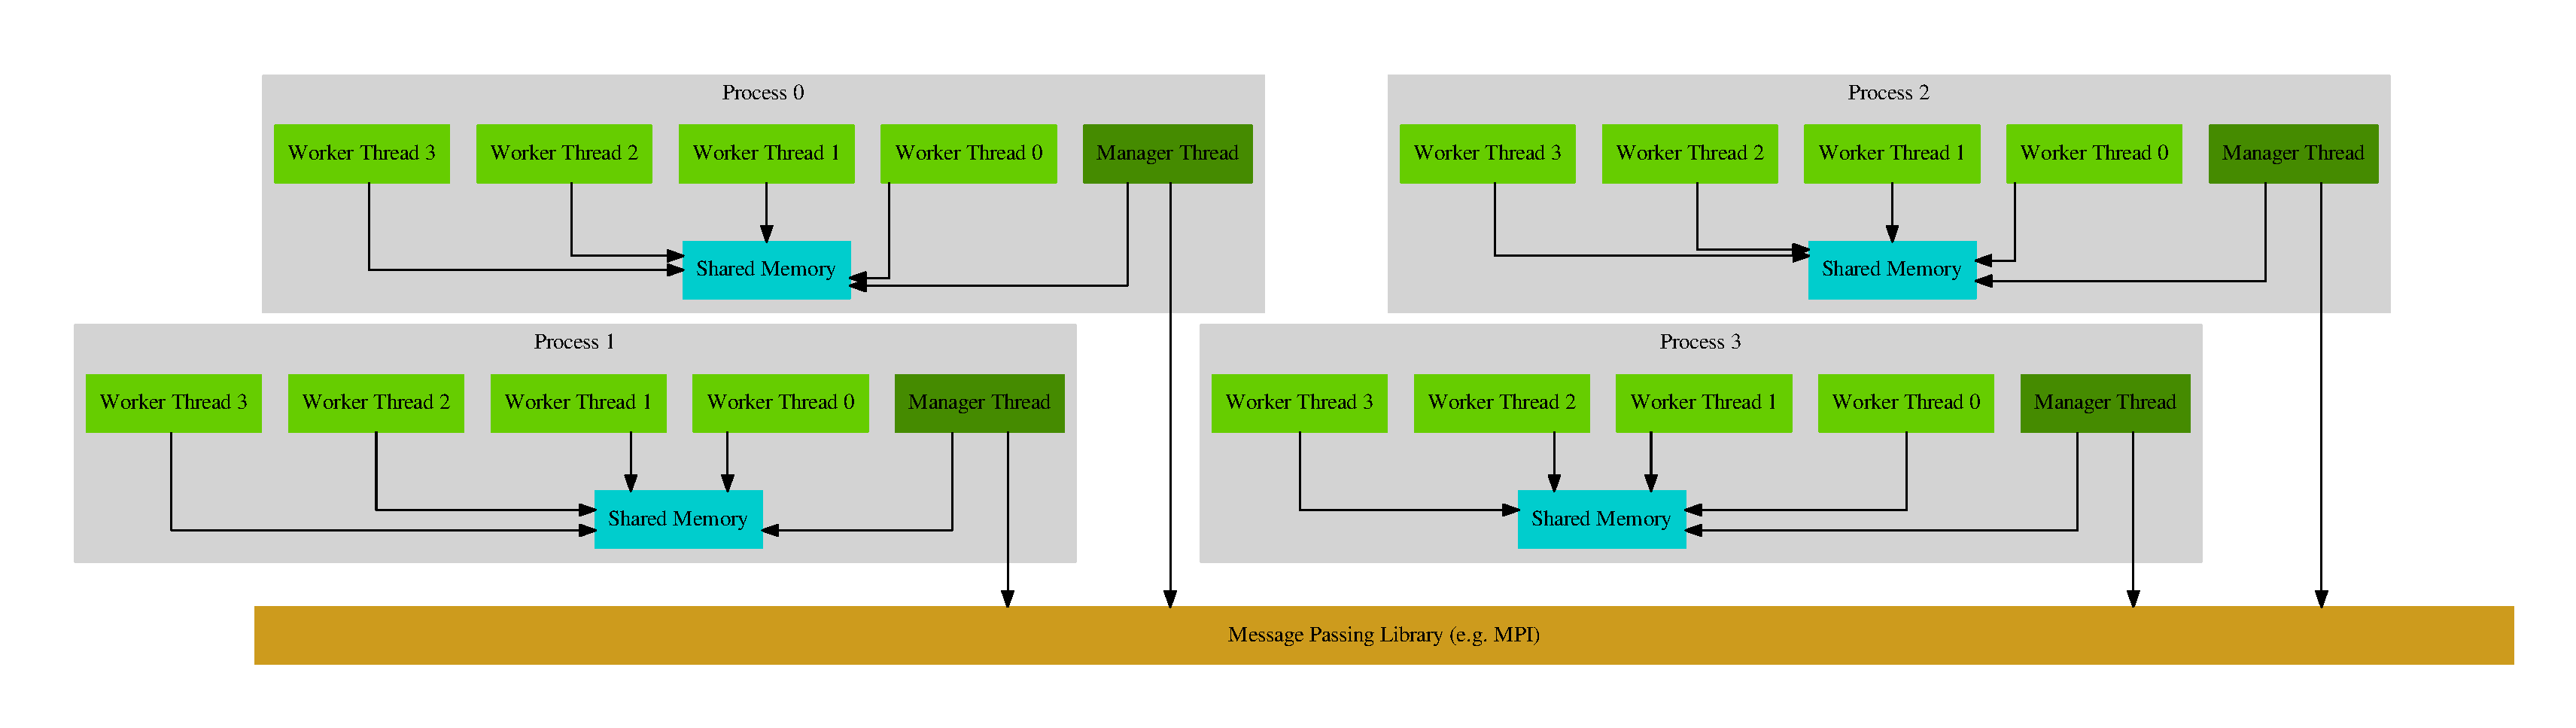
\includegraphics[width=\textwidth]{figs/graphviz/warped_communication.pdf}
    \caption{Communication Model of \textsc{warped2}}\label{warped2_communication}
\end{figure}

%% Scheduling
\noindent
This communication model not only allows for high scalability and reduced communication
overhead within processes, but allows time warp simulations to follow the critical path better
since the worker threads can share a scheduling data structure to process events from.
Fewer scheduling data structures creates a bottleneck since multiple worker threads cannot
access them simultaneously without race conditions. On the other hand, more scheduling
data structures allows more concurrency but spreads out the critical path of execution,
allowing more rollbacks.

%% Partitioning
To further reduce any communication overheads in both message passing and shared memorory
communication, partitioning the work between processes will also be explored. Partitioning
the work in a parallel discrete event simulation is achieved by simply partitioning the
LPs. In \textsc{warped2}, a two phase partitioning scheme will be explored. The first phase
is for partitiong LPs among processes in order to minimize communication and the second
phase is for further partioning the LPs in a process to the event scheduling data structure
which should localize LP communication among worker threads and reduce rollbacks.

%% GVT and Termination
The combination of shared memory and message passing communication does create some
complications in the implementation of a time warp system. GVT and termination detection
algorithms are usually designed for either shared memory or message passing but not both.
Using a single message passing algorithm between worker threads and processes would mean
that some kind of message passing scheme would have to be implemented for worker threads
to communicate. This scheme would still use shared memory for message communication but
would still have the overheads of explicit message passing. On the contrary, it is possible
to have a single shared memory algorithm that extends to distributed memory systems but
would require a shared virtual memory system. A shared virtual memory system would still
have to transparently use message passing to achieve synchronization. For these reasons,
the GVT and termination algorithms developed for \textsc{warped2} include a message
passing algorithm and a shared memory algorithm that work in conjunction.

\section{Thesis Overview}

The remainder of this thesis is organized as follows:

Chapter \ref{background} contains some background information on parallel simulation and
parallel computing that is used in this thesis.

Chapter \ref{related_work} reviews several of the prominent parallel simulation kernels
that use the Time Warp synchronization protocol.  The software architecture and target
compute platforms for each is described.

Chapter \ref{warped2_overview} introduces the software architecture and modeling API for
the \textsc{warped2} simulation kernel.

Chapter \ref{warped2_ds} describes the pending event set data structures used within
the \textsc{warped2} kernel and provides some preliminary results in finding the best
configurations for various models.

Chapter \ref{gvt_termination} descibes various GVT and termination detection algorithms that
have been used explains the algorithms used in \textsc{warped2}. This chapter also provides
some preliminary results in determining the best configurations for these algorithms.

Chapter \ref{memory_management} analyzes techniques for managing memory efficiently. This
includes state saving techniques, fossil collection, and GVT period. Some preliminary results
are also shown for various configurations.

Chapter \ref{experimental_analysis}

Chapter \ref{big_little_platform}

Finally, Chapter \ref{conclude} contains some concluding remarks and suggestions for future
research.



\chapter{Background}\label{background}

This chapter describes some of the basics of Parallel Discrete Event Simulation (PDES) with
a focus on the Time Warp mechanism. Then a brief overview of parallel architectures and
parallel communication models and their strengths and weaknesses are compared. Lastly, the
big.LITTLE platform is introduced and some different scheduling/switching mechanisms are
described.

\section{Discrete Event Simulation}

Discrete Event Simulation (DES) is a method of modeling the execution of a physical system
with a sequence of events that occur at discrete time intervals. A Discrete Event Simulation
typically contains three main data structures

\begin{description}
    \item[State variables: ] A set of variables that describe the current state of the system.
    \item[Simulation Clock: ] A clock to measure the progress of the simulation and determine
        the order of event processing.
    \item[Pending Event Set: ] A set of future events that are waiting to be procesed.
\end{description}

\noindent
A \emph{Simulation Model} describes a physical system by a set of \emph{Logical Processes}
(LP's). Each LP corresponds to a physical process that is part of the physical system. The
LP's interact with timestamped events that dictate the simulation time that the event should
be processed. With each event that occurs, and only when an event occurs, the state of the
system is updated.

In a \emph{Sequential} Discrete Event Simulation only one event is processed at a time.
All pending events are kept in a single list which is sorted by timestamp. The next event
to be processed is always the one with lowest timestamp. Each successive event updates the
state of the system, advances the simulation clock, and possibly produces new future events.
This is clearly not very efficient for large simulations. This method can be improved by
realizing that events for different LP's are independant and will only affect the state for
a single LP.

\section{Parallel Discrete Event Simulation}

\emph{Parallel} Discrete Event Simulation (PDES) is a method running a discrete event
simulation on a parallel computer which could be a shared-memory multiprocessor, a distributed
memory system such as cluster or NUMA system, or a combination of both. In a parallel
discrete event simulation the state of the system is usually split among the logical
processes so that each one contains a portion of system's state without any sharing of
state variables\cite{fujimoto-90}. In addition to each logical process having it's own
separate state, the logical processes also have seperate simulation clocks and pending
event sets. Event's from different LP's can then be processed concurrently without the
need to worry about sharing state variables and the model can be viewed as concurrent
processes operating independantly which contribute to the overall progression of the
simulation. This has the potential to increase performance significantly; However, it is
possible that events at a receiving LP can be received and processed out of order, violating
causality. These \emph{causality errors} can occur because of the independant nature of the
logical processes and because the LP's can be processing events at different rates.
Causality errors can produce incorrect changes in state variables and incorrect events to
be sent to other LP's. Parallel Discrete Event Simulation techniques can be categorized in
terms of how causality errors are handled. \emph{Conservative} approaches use methods to
detect when possible causality errors might occur and prevent them from ever occuring.
\emph{Optimistic} approaches, on the other hand, allow causality errors to occur but use
methods to detect and recover from the errors. Generally, the simulation models can be
developed without the knowledge of the underlying simulation mechanism. The simulation
mechanism is usually implemented in a self-contained module which provides an API for the
models and is commonly referred to as the \emph{kernel} or \emph{executive}. For the remainder
of this text, only optimistic methods will be discussed, specifically the Time Warp mechanism
which is the most widely used optimistic mechanism used in practice.

\subsection{Time Warp}

The Time Warp mechanism is an optimistic method of simulation which is based on the virtual
time paradigm\cite{jefferson-85}. \emph{Virtual Time} provides a method of ordering events
in distributed systems which are not described by real time such as a simulation. When used
for parallel discrete event simulation, Virtual Time is synonymous with simulation time.
The current time of an LP's simulation clock in Time Warp is called the \emph{Local Virtual
Time} (LVT).

When an a causality error is detected at an LP (next event to be processed is less than the
simulation time) the effects of the incorrectly processed event(s) must be undone. The process
of undoing the effects is called a \emph{rollback} and the event that triggers a rollback
is called a \emph{straggler event}. When a straggler event is detected at an LP, the first
step taken during the rollback is to restore the LP's state back to a previous state before
the incorrect event(s) were processed. Then the LP must "unsend" the events that were
incorrectly sent by sending \emph{negative events} or \emph{anti-messages}. The negative
event, when received by the receiving LP will stop the corresponding positive event from
being processed or if the corresponding positive message has already been processed at
the receiving LP then that LP must also rollback. This processes recursively occurs until
all causality errors are corrected. The negative messages are never processed as normal
events but serve only to annhilate an generated event produced by an incorrectly processed
event (causality error).

Jefferson\cite{jefferson-85} describes how to support rollbacks with three main data structures:

\begin{enumerate}
    \item Input Queue
    \item Output Queue
    \item State Queue
\end{enumerate}

\noindent
Every LP will have a seperate input queue, output queue, and state queues. The input
queue contains the unprocessed and processed events for the LP that it belongs to. The
input queue must be sorted in timestamp order and the LP's must always process from the
lowest unprocessed event. The LVT is always the largest timestamped processed event and
is used to detect a straggler event. The output queue contains the events that have been
sent by the LP that it belongs to which will allow the LP to send anti-messages during a
rollback. The state queue contains previous states of the LP and allows the proper states
to be restored during a rollback.

The \emph{Global Virtual Time} (GVT) of the simulation at a given point during the simulation
is the minimum of all unprocessed events and the send times of all events that have been
sent but not received\cite{jefferson-85}. There are numerous algorithms for determining
the GVT which will be discussed further in chapter\ref{gvt_termination}. LP's cannot send
events that are less than their LVT value and so the GVT acts as a lower bound on how far
a rollback can occur. Because no LP's will ever rollback past the GVT value, it is often
used to free memory that is no longer needed for the events in the input and output queues
and the states in the state queue that have timestamps less than the GVT as well as committing
I/O operations that cannot be undone. This process of freeing memory and committing I/O
operations is known as \emph{fossil collection}. Fossil collection does not have to be based
on the GVT and several other methods of fossil collection have been developed which will
also be discussed more in chapter \ref{memory_management}.

The need to save the state of the LP's is one of the fundamental overheads in the Time Warp
mechanism in terms of both the amount of time it takes to copy the LP's states to save them
and the amount of memory that must be used to store them. Because of this, a number of
different approaches have been developed to reduce the overhead of state saving such as
periodic state saving, incremental state saving, and reverse computation.

\section{Parallel Systems Architectures}

Systems that support parallel processing come in many forms. They can generally be
characterized by how processors and memories are grouped together. Shared memory
systems are a single machine which share a common address space which can have a single
physical memory unit or multiple memory units. On the other hand, a cluster is a system
comprised of multiple machines with seperate address spaces. 

\subsection{Shared Memory Multiprocessor Systems}

\paragraph{A Symmetric Multiprocessor (SMP)} is a type of shared memory multiprocessor
system where each processor has uniform access to a single shared memory through a common
bus. SMP systems cannot scale very large due to increasing contention as the number of
processors increasing and for this reason, they usually have 8 or fewer processors.
To increase available bandwidth in the system, each processor usually has one or two
levels of private caches as well as a shared cache which act as a way limit the number of
memory accesses. Figure \ref{smp} illustrates what a typical SMP system looks might look
like.

\begin{figure}[H]
    \centering
    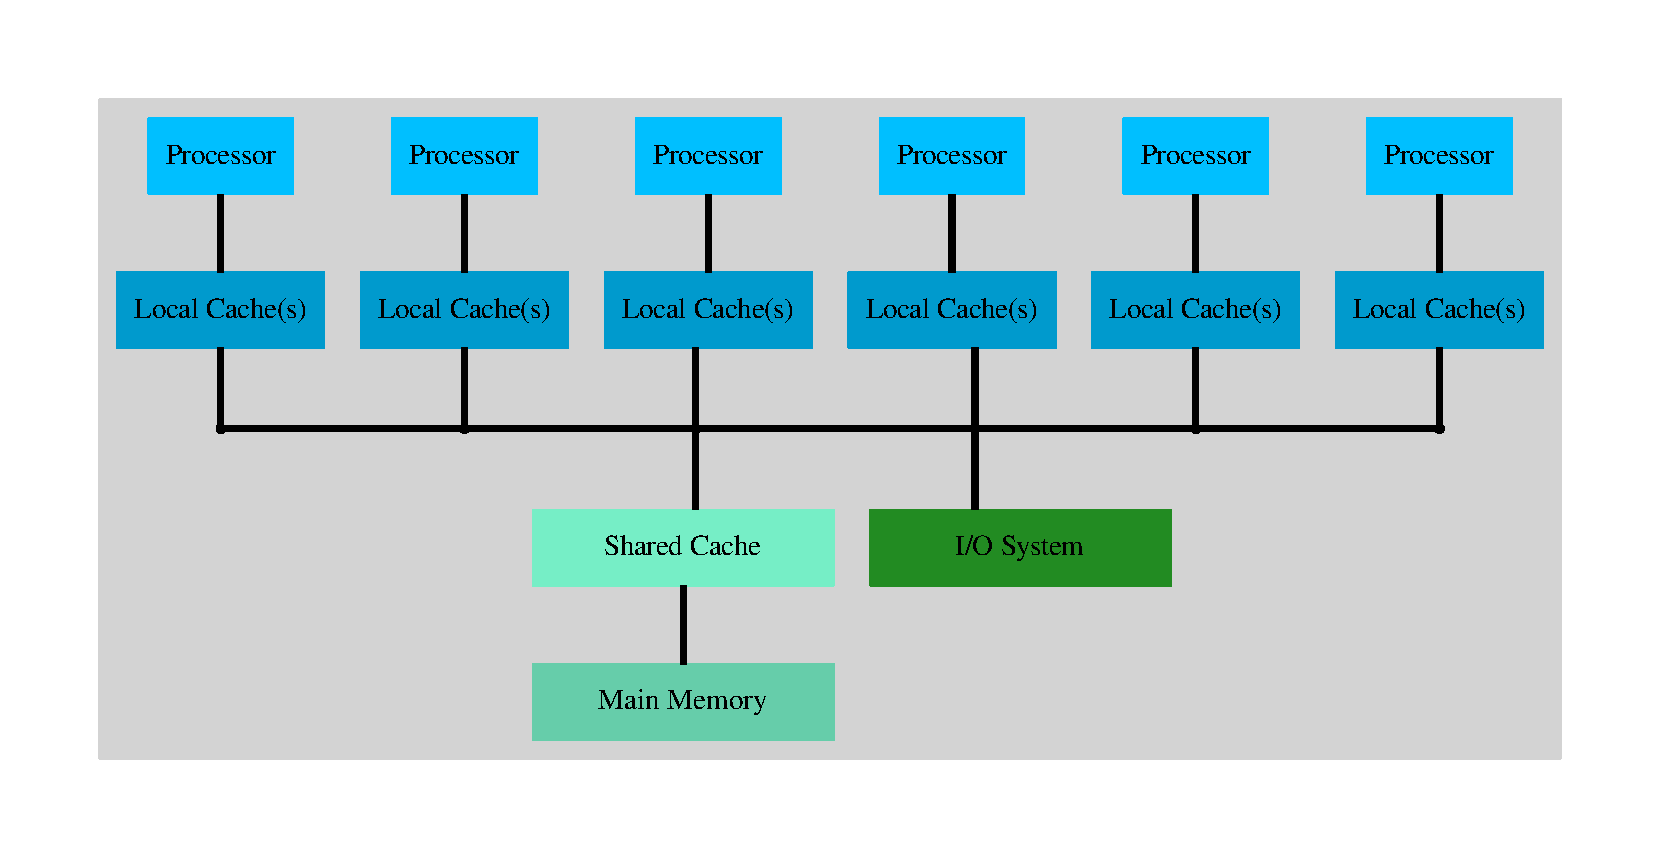
\includegraphics[width=0.75\textwidth]{figs/graphviz/smp.pdf}
    \caption{SMP System}\label{smp}
\end{figure}

\paragraph{A Distributed Shared Memory} sytem, also known as a Non-Uniform Memory Access
(NUMA) system has mulitple memories that are distributed. In these systems, the memories are
stilled shared between processors, but access to different memories may take different amounts
of time. An interconnection network connects processors and memories together with one or
more processors per memory. Because memory access times can vary, software on NUMA systems
usually try to keep memory accesses local to a processor. However, NUMA systems can scale
much larger than SMP systems because contention to single memory does not necessarily increase
with an increasing number of processors. Figure \ref{distributed} illustrates what a typical
NUMA system might look like.

\begin{figure}[H]
    \centering
    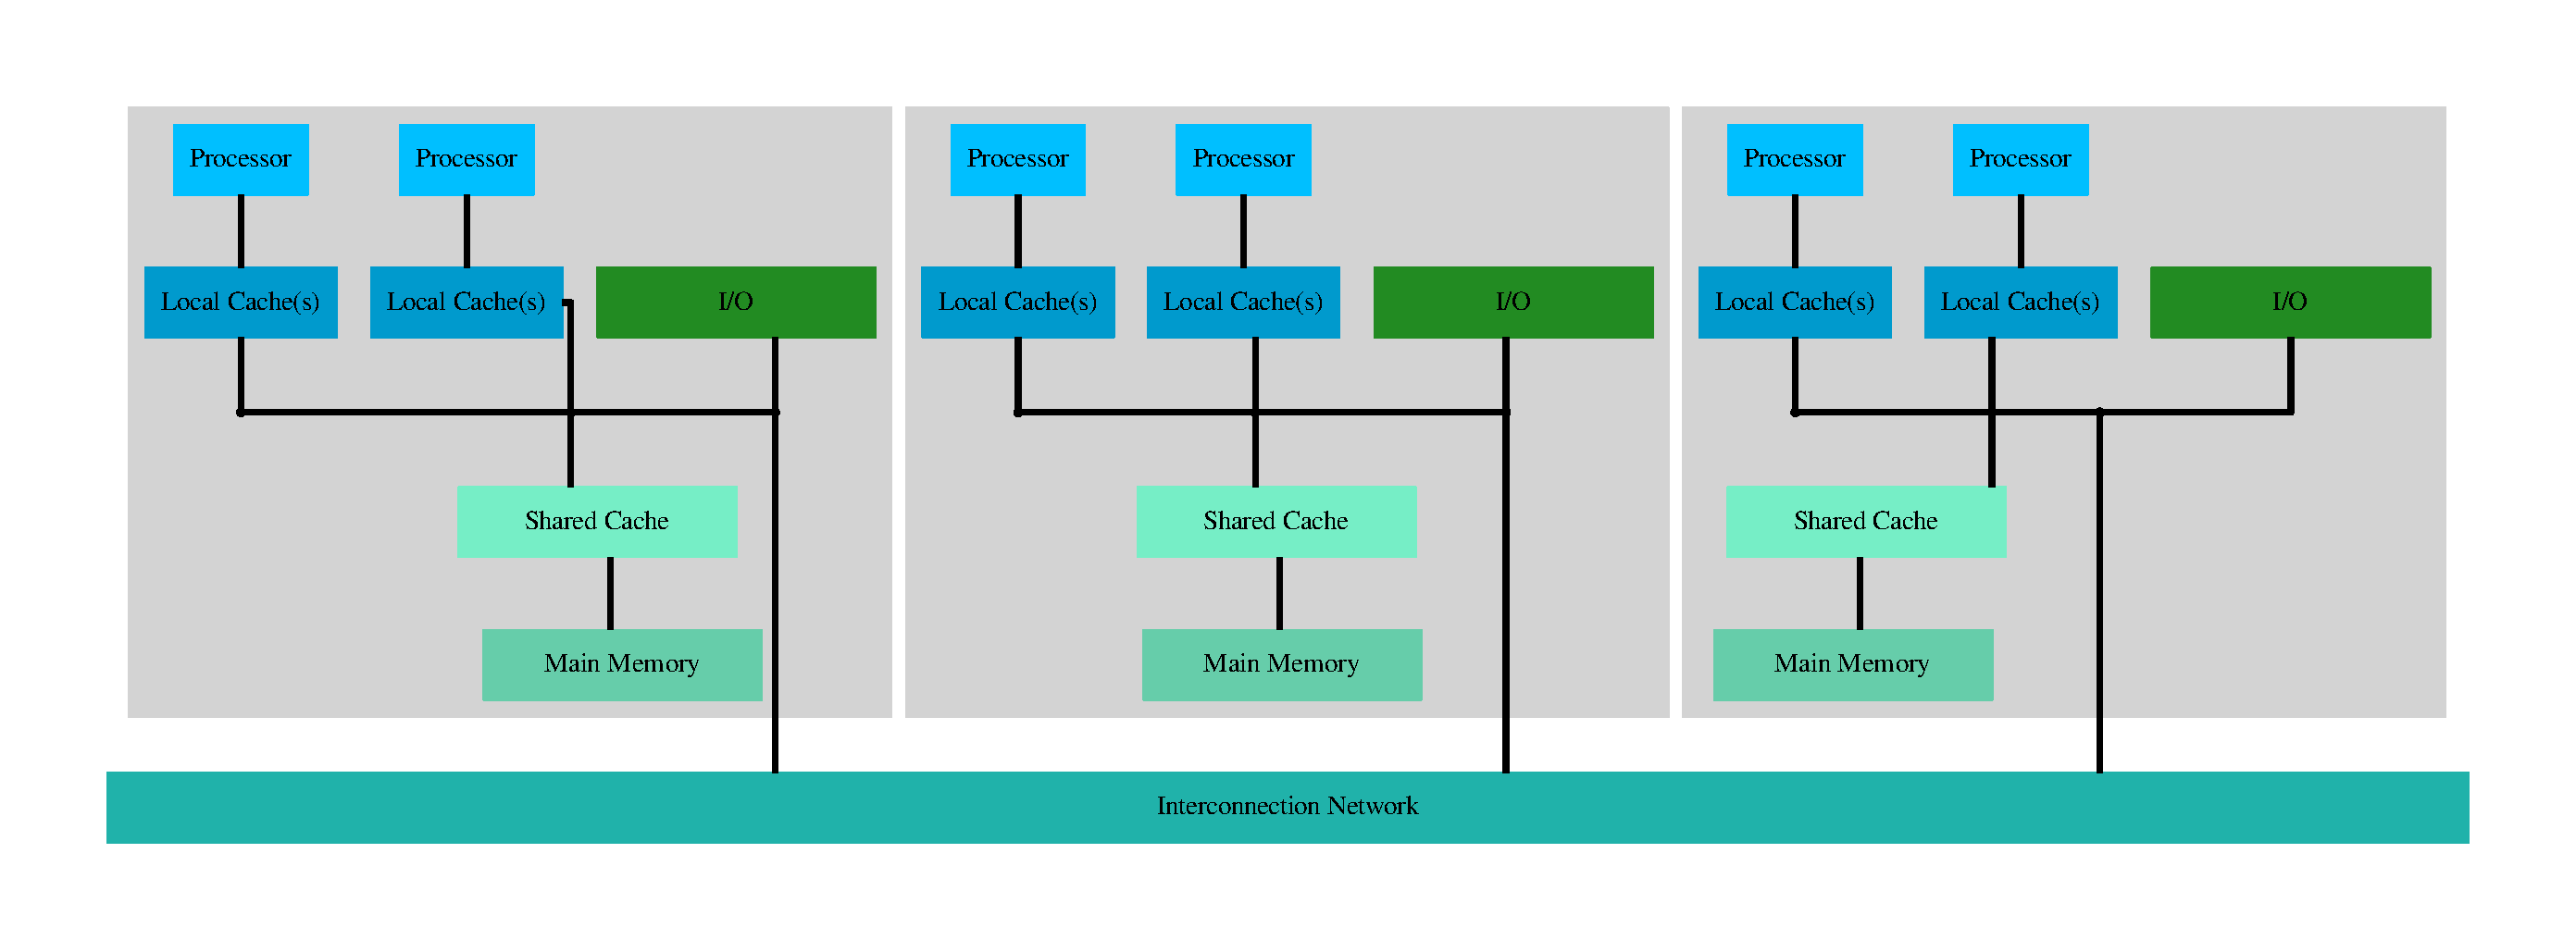
\includegraphics[width=\textwidth]{figs/graphviz/distributed.pdf}
    \caption{NUMA System}\label{distributed}
\end{figure}

\subsection{Clustered Systems}

\paragraph{A Beowulf Cluster} is a type of cluster which appears to the user as a single
machine but is actually a loosely coupled set of machines connected together over a local
network. A single program is executed by all machines concurrently by launching multiple
processes on each machine. A program written for a beowulf cluster typically use some type
of message passing to communicate among processes and is typically written with parallel
communication software such as MPI or PVM. Figure \ref{beowulf} illustrates a common realization
of a beowulf cluster.

\begin{figure}[H]
    \centering
    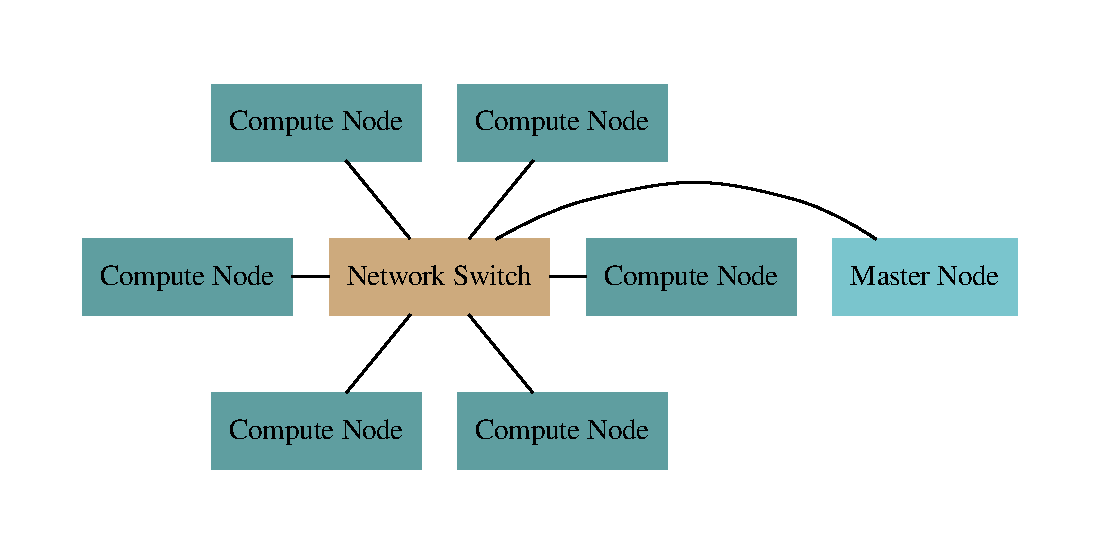
\includegraphics[width=0.6\textwidth]{figs/graphviz/beowulf.pdf}
    \caption{Beowulf Cluster}\label{beowulf}
\end{figure}

\section{Parallel Systems Communication}

Parallel applications are composed of multiple workers that operate independantly in parallel
and may have to exchange information. The workers in a parallel application can be a process,
thread, or any other type of execution context and can be within a shared memory system or a
cluster or any type of parallel system. Workers can communicate by either sending explicitly
passing messages to each other by means of well defined message formats or by using shared
data structures that all workers can access. The former method of communication is known as
\emph{message passing} and the latter method of communication is known as \emph{shared memory}
communication. Both communication methods are fundamentally different and both have strengths
and weaknesses.

\subsection{Message Passing}

In a message passing system, workers are completely isolated in different address spaces
and communicate only through serialized messages. The formats of the messages must be
defined so that the message can be serialized and deserialized by the sender and the reciever,
respectively. Message passing can either be synchronous or asynchronous. With synchronous
message passing, the send/receive operations must be done in a specific order so that the
sender/receiver workers operate together in a synchronized fashion. The send operation at
the sender will block until the message is received at the reciever and the receive operation
at the receiver will block until the message is fully received. That means the every worker
must follow a predictable communication pattern. Workers cannot continue other operations
during communication operations and may slow down the whole system. On the other hand,
asynchronous communication allows workers to start a send and recieve operations and immediately
continue without blocking. To allow this, temporary queues must be used to hold pending
operations. The workers do not have to follow a predictable communication pattern in this
case because the messages will be queued and can be processed at any time and in any order.
The main advantage of message passing is that the number of workers can be scaled to any size
as long as the work is partitioned in the right way. Also, he workers can execute in address
spaces on different machines and communicate over a local network connection. The biggest
disadvantage, however, is an increased communication latency which can be vary large compared
to the speed of computation. This makes message passing especially hard for fine-grained
parallel applications. An illustration of simple message passing is shown in figure
\ref{communication}.

\subsubsection{Message Passing Interface (MPI)}

MPI\cite{Forum:1994:MMI:898758} is an extensive message passing API specification for parallel
applications and supports both synchronous and asychronous forms of communication. It is
a standard specification for developers and MPI users and many current implementations exist.
The most widely used implementations used in practice include MPICH and OpenMPI.

\subsection{Shared Memory}

The workers in a parallel application can also share a common address space and communicate
through shared data structures. The producer worker will insert data directly into the data
structure and the consumer worker will remove the data and use it. This takes much less time
to transmit data than with a message passing scheme. However, access to the shared data
structures must be protected so that multiple workers do not simultaneously access the same
data which could cause unpredictable results. Access to the data structures is usually enforced
using lock synchronization mechanisms that protect entire sections of code that are executed by
different workers and can end up accessing the same data structures such as mutexes or semaphores.
Shared memory data structures may suffer from performance if lots of workers contend for the
lock at the same time. For this reason, it is very hard to scale systems that use only shared
memory as a means of communication. An illustration of a simple shared memory system is show
in figure \ref{communication}.

\begin{figure}[H]
    \centering
    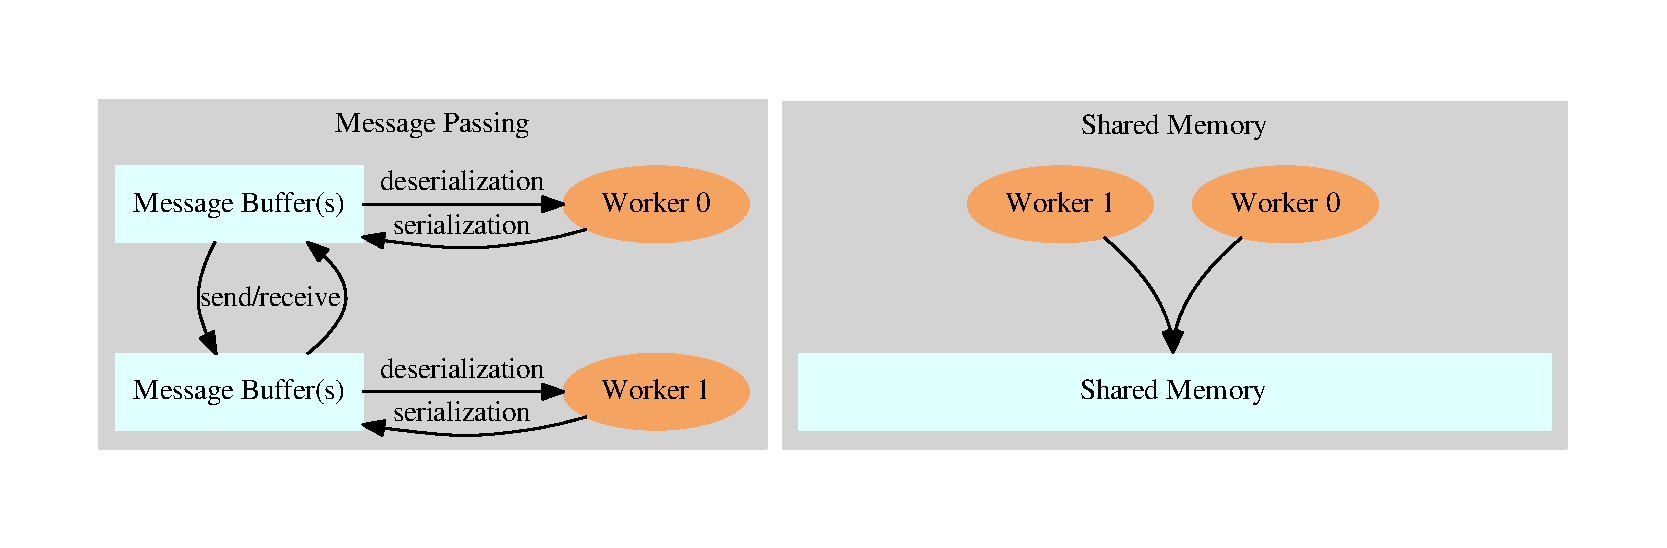
\includegraphics[width=\textwidth]{figs/graphviz/parallel_communication.pdf}
    \caption{Message Passing and Shared Memory Communication}\label{communication}
\end{figure}



\chapter{Related Work}\label{related_work}

This chapter give an overview of some of the most popular Time Warp implementations. For each
impementation the design will be described at a high level with a focus on the target
architecture. The featured data structures and algorithms for each will also be described
as well as the strengths and weaknesses.

\section{Georgia Tech Time Warp (GTW)}

Georgia Tech Time Warp wass a general purpose Time Warp Simulator designed specifically for
shared memory multiprocessors. It is not used anymore, however, because it was only written
to target SparcStation and SGI PowerChallenge which are now obsolete. Although GTW is not
used any more, it's design has influenced the design of other simulators that are still used
widely in practice. GTW simulation models run in a single processes, multi-threaded environment
and uses only shared memory to communicate between threads that are bound to single processor.

The LP's for all models are statically allocated to a single thread so that events for the
LP's are processed only on a single processor. The pending event set is distributed among
threads with each having its own data structures for the set of LPs that belong to it.
Since the threads can only run on a single processor, the data structures also belong to a
singl processor. The pending event set for each processor consists of three main data structures
listed below\cite{das-94}:

\begin{enumerate}
    \item The \emph{Message Queue} is a linked list that contains positive messages that
        are destined for the LP's mapped to the owning processor. Access to the message
        queue must be synchronized because it can be accessed by tasks running on any processor.
    \item The \emph{Cancel Queue} is a linked list that serves exactly the same purpose as
        the message queue except that it containes only negative messages(anti-messages).
        Access to this queue must also be synchronized.
    \item The \emph{Event Queue} is used to hold unprocessed and processed events and is
        directly used to schedule events to be processed. The event queue is actually made
        up of different data structures, one for processed events and one for unprocessed
        events. The processed events are contained within a doubly linked list and the
        unprocessed events are contained within a priority queue which can be configured to
        be either a calendar queue or a skew heap depending on a user configuration.
\end{enumerate}

\noindent
When messages are sent between LP's, they are inserted directly in the message queue or
the cancel queue depending on whether they are positive or negative. Each thread processes events
by first moving events from the message queue to the event queue and processing rollbacks. Then,
the messages from the cancel queue are removed and cancellations are processed and any more
rollbacks are processed. One or more of the smallest events from the event queue are then processed
and added to the processed event list. This procedure is repeated over and over again by all processors.
Psuedocode for the main event processing loop in GTW is show in figure \ref{gtw_processing}.

\begin{algorithm}
\DontPrintSemicolon
\SetAlgoVlined
    \While{eventQ is not empty} {
        move messages from MsgQ to EvQ and process any rollbacks\;
        remove anti-messages from CanQ, process annihilations and rollbacks\;
        remove N smallest timestamped events E from EvQ\;
        process the N events\;
    }
\caption{GTW Main Event Processing Loop\cite{das-94}\cite{fujimoto-94}\label{gtw_processing}}
\end{algorithm}

\noindent
To avoid accessing the message queues and cancel queues too often, which is a contention point,
a larger value of N can be used. GTW calls this batch processing and N is the batch interval.
With batch processing, multiple events will be processed at a time without processing any
rollbacks or cancellations.

Since GTW is only uses shared memory communication, anti-messages do not need to be explicitly
sent. Only a pointer to the event that needs to be cancelled is necessary. Fujimoto calls
this method \emph{direct cancellation}. Also by only using shared memory, GVT can be calculated
very quickly using shared data structures instead of passing messages around to all processors.
The downfall of GTW, however is that it was limited to only a single multiprocessor machine and
it was only designed and optimized for specific architectures.

GTW also imposed some unnecessary requirements for the developer of particular simulation
models. The partitioning of the LP's among processors must be done in the simulation model
during initialization. That means that the model developer must understand some the features of
the underlying architecture such as the number of processors, to effectively partition the
LP's. Furthermore, the initial partitioning of the LP's is hard to dynamically balance during
the simulation because there are no seperate input queues for each LP but rather a single
message queue to hold all unprocessed events for each processor.

\section{Clustered Time Warp (CTW)}

Clustered Time Warp\cite{avril-95} (CTW) uses a hybrid approach by processing events within
a \emph{cluster} of LP's sequentially and using the Time Warp mechanism between the clusters.
This design was chosen because it works well for digital logic simulation which tend to have
localized computation within a group of LP's. Furthermore, digital logic simulation tends to
have low computational granularity and lot's of LP's which can lead to a lot of rollbacks
and a large memory footprint in a traditional Time Warp simulator. CTW is implemented for
shared memory multiprocessors but only uses shared memory for use with a custom message passing
system so that it can better support NUMA architectures. It is not designed for use on a
network of machines such as a beowulf cluster.

Each cluster of LPs has a timezone table, an output queue, and a set of LP's which each have an
input queue and a state queue. The timezones in the timezone table are divided by timestamps
of the events received from LP's on different clusters. Whenever an event is received from
a remote cluster, a new timezone is added. Only a single output queue is needed per cluster
because anti-messages can only be sent between clusters and not between LP's on the same
cluster.

When a straggler event arrives at a cluster, all of the LP's that have processed events that
are greater than the timestamp of the straggler will be rolled back. This rollback scheme is
called \emph{clustered rollback}. The alternative to clustered rollback is \emph{local
rollback}. In a local rollback scheme the straggler event would be inserted into the receiver
LP's input queue and the LP will roll back when it is detected. Although clustered rollbacks
may cause some LP's to be rolled back unnecessarily leading to slower compuation, the
approach was chosen for CTW because processed events will not have to be saved which
requires less memory.

CTW uses a form of infrequent state savings with the timezone table used to determine the
frequency. When an event is about to processed for an LP, the timezone of the last processed
event is looked up and if event that is about to be processed is in a different timezone then
the state is saved. This approach in which all LP's save their state every time an event is
processed in a new timezone regardless of whether it receives an event from a remote cluster
is called \emph{local checkpointing}. This method reduces the state saving frequency more
than a \emph{clustered checkpointing} approach in which only the LP that receives an event
from a remote cluster saves its state. The local checkpointing approach was chosen for CTW
because a larger state saving frequency can increase rollback computation and it can even
lead to more memory consumption because more events must be saved for coast forwarding
during state restoration.

\section{Rensselaer's Optimistic Simulation System (ROSS)}

ROSS\cite{carothers-00} is a general purpose simulator that is capable of running both
conservatively and optimistically synchronized parallel simulations as well as sequential
simulations. It is most often used for optimistic parallel simulations which is achieved
with the time warp mechanism. ROSS started as a reimplementation of GTW and is still
modeled after it but has had many enhancesments. The same basic event scheduling mechanism is
used but ROSS supports different priority queue implementations and different algorithms
are used for fossil collection, state saving, and gvt calculation. In addition, ROSS uses
processes instead of threads and uses message passing explicitly with MPI instead of shared
memory for communication among the processes.

Just as in GTW, ROSS maps every LP to a process and each process contains its own pending
event set structures. No locks are needed explicity within each process because there are
no shared data structures among processes. The data structures are very similar to those
used in GTW but have a different naming convention. The main data structures in ROSS are:

\begin{enumerate}
    \item The \emph{Event Queue} is analogous to the message queue in GTW. It contains the
        positive events for all LP's in the corresponding process. In addition, an event
        queue is used to hold all remote events regardless of whether it is positive or
        negative. The event queue is implemented as a linked list.
    \item The \emph{Cancel Queue} is a linked list which is used to hold negative events
        for all LP's for the corresponding process. The cancel queue is used in the exact
        same way as GTW except that no locks are necessary.
    \item The \emph{Priority Queue} is analogous to the unprocessed event queue in GTW and
        contains events in timestamp order. ROSS also allows the priority queue to be
        implemented as a calendar queue, heap, splay tree, or avl tree depending on user
        configuration.
\end{enumerate}

\section{\textsc{warped}}

\textsc{warped} is the predecessor of \textsc{warped2} and serves as the basis for the design
and architecture of \textsc{warped2}. \textsc{warped} started as a completely processed-based
solution with only message passing for communication. Eventually, with the development of
multicore processors, each process was extended into multiple threads to further enhance
concurrent processing of events. Over the years, with many students developing new algorithms
in \textsc{warped2}, the complexity of \textsc{warped} became unmaintainable, mainly because
of the great deal of indirection which, although made for a super configurable and modular
design, became too complex for new students to learn it and enhance it.

\section{Others}

\subsection{The ROme OpTimistic Simulator (ROOT-Sim)}

ROOT-Sim is another general purpose Time Warp Simulator that uses message passing via MPI
\cite{pellegrini-11}. Like \textsc{warped}, ROOT-Sim is a more classic Time Warp
implementation with each LP having their own input queues, and output queues. What sets
ROOT-Sim apart from other time warp simulators is the internal instrumentation tool, Dynamic
Memory Logger and Restorer (DyMeLoR) that can optimize memory usage. DyMeLoR can determine
whether the simulation models are better fit for copy-state saving or incremental state
saving and transparently switch between them during runtime. Another service that ROOT-Sim
offers is the Committed and Consistent Global Snapshot (CCGS). After each GVT calculation,
ROOT-Sim transparently rebuilds a global snapshot of all LP states. Each LP can access its
portion of the global snapshot on every GVT calculation. With this service, a simulation
model can implement any custom global snapshot algorithm.

\subsection{ROSS-MT}

ROSS-MT\cite{jagtap-12} is a multi-threaded version of ROSS which is optimized to use shared
memory to communicate among threads. The use of message passing with MPI was completely
removed and all events are sent by direct insertion into the event queues. To reduce the
added contention on the event queues, they are further divided by possible senders. ROSS-MT
also optimizes the free memory lists so that they are more NUMA aware. Instead of allocating
memory from the receiver processors free list, it is allocated from the senders free list.
Furthermore, a LIFO approach is taken to improve cache reuse.



\chapter{The \textsc{warped2} Simulation Kernel}\label{warped2_overview}

This chapter describes the software architecture of the \textsc{warped2} simulation kernel.
The main compenents are described and the dependencies between each of them. The modeling API
is also described and an example model is shown to illustrate the API.

\section{The Software Architecture of \textsc{warped2}}

The \textsc{warped2} simulation kernel uses a modular design to make it more configurable,
extendable, and maintainable. All components are configured and created at startup individually
and subcomponents are accessed through pointers. Furthermore, \textsc{warped2} is written in
C++ so each component can also be an object of derived subclass that implement a well-defined
interface by a base class. The main central component is the event dispatcher which is responsible
for calling the LP callback methods during the course of the simulation as well as determing
when rollbacks and cancellation is necessary and carrying them out. The main components and
how they depend on eachother are illustrated in figure \ref{warped2_architecture}.

\begin{figure}[H]
    \centering
    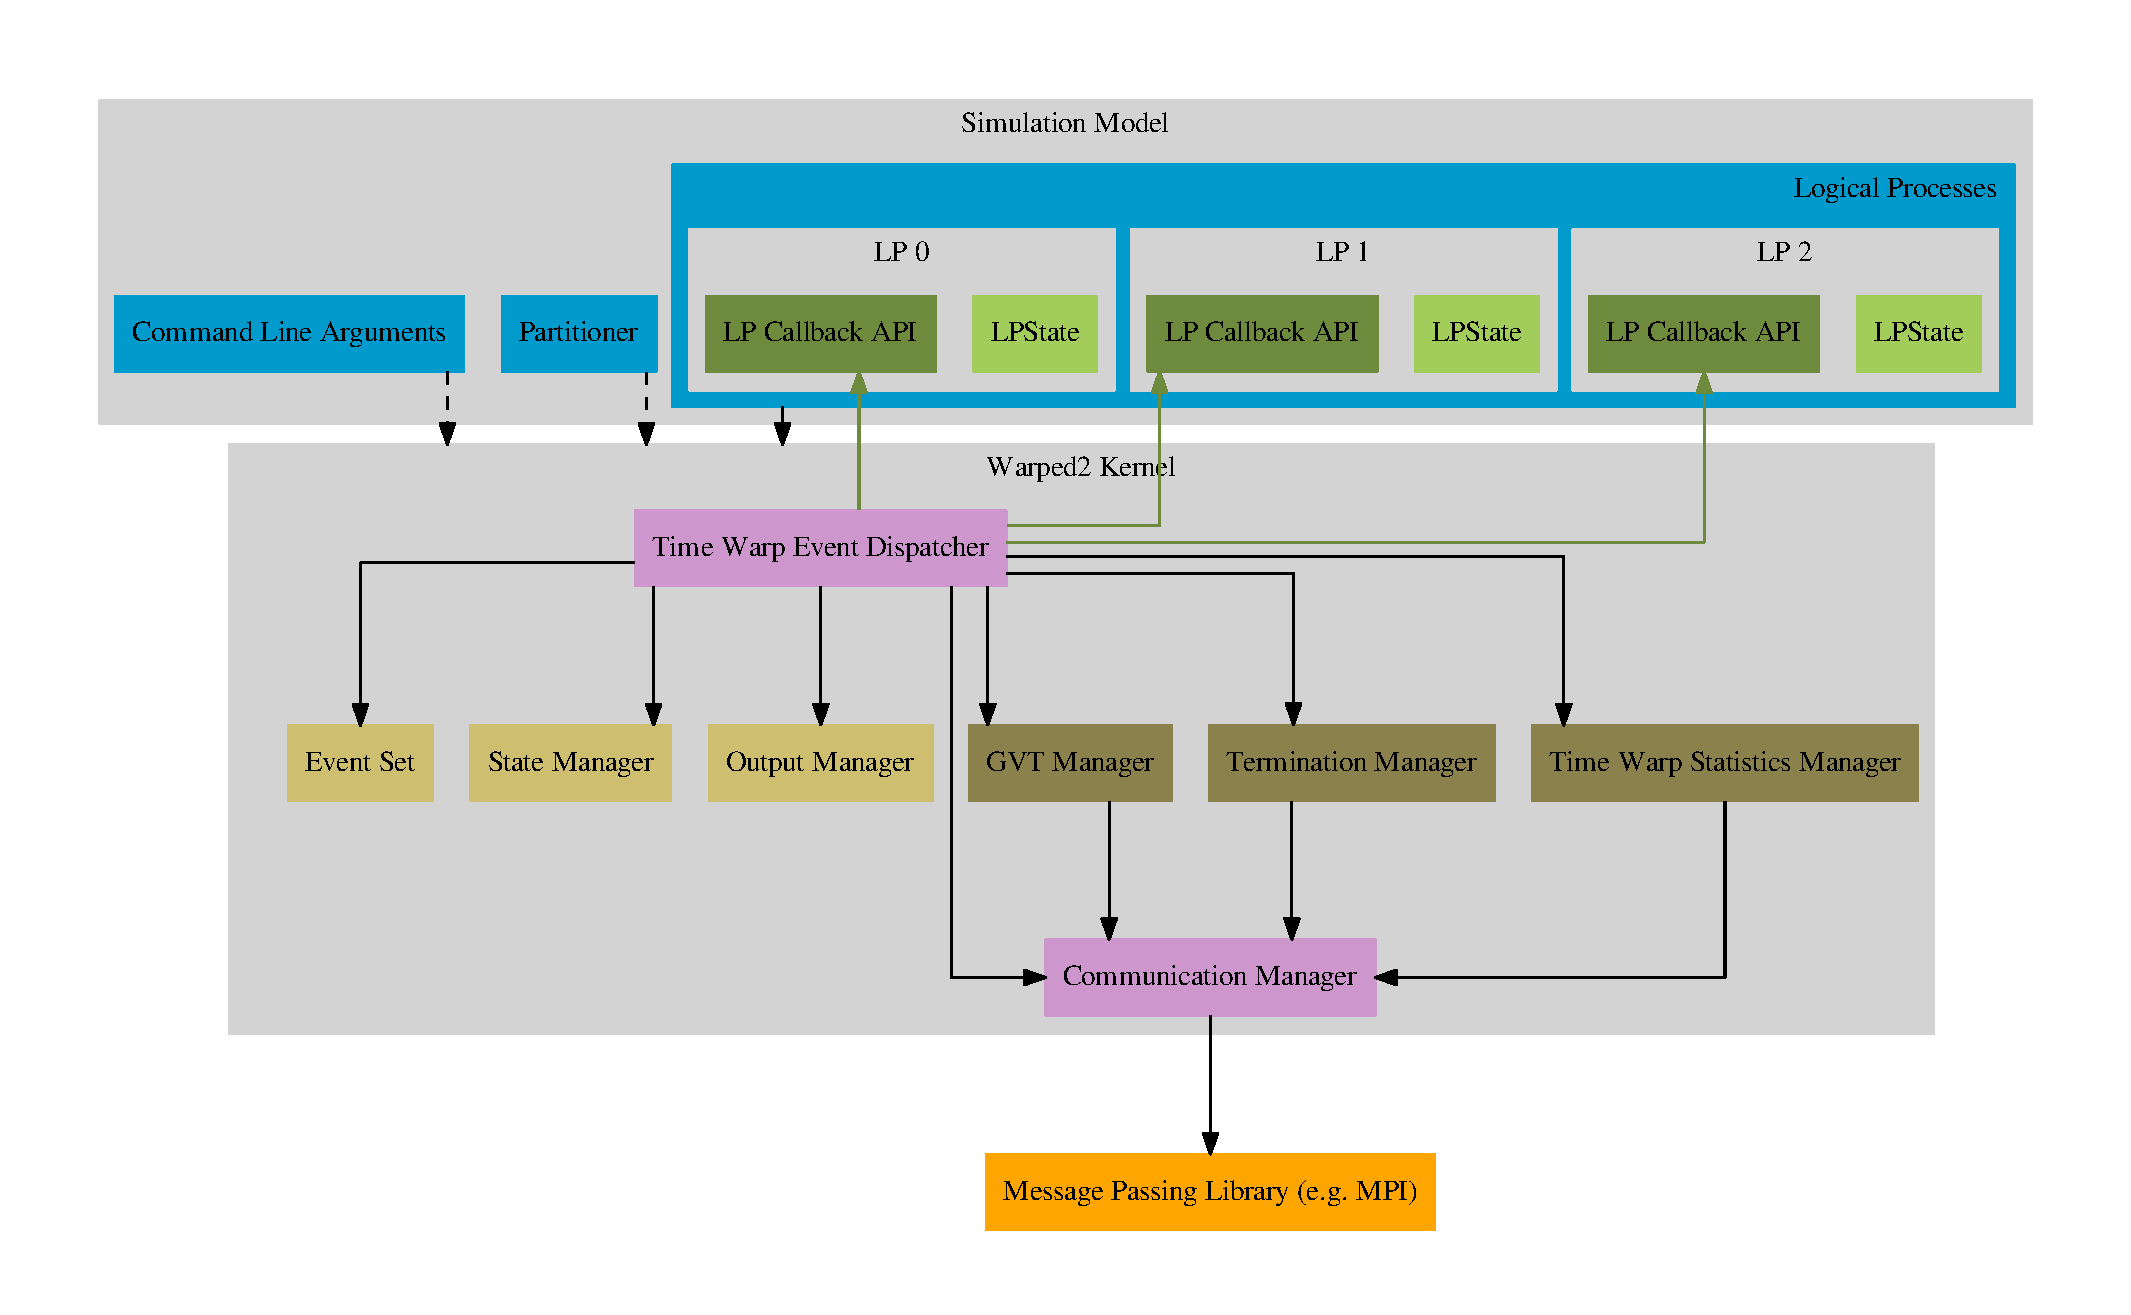
\includegraphics[width=\textwidth]{figs/graphviz/warped2_overview.pdf}
    \caption{Time Warp Components in \textsc{warped2}}\label{warped2_architecture}
\end{figure}

Warped2 also supports a sequential event dispatcher. The sequential event dispatcher, however
does not depend on any other components and just contains a single list of all events since
only a single event is processed at a time.

The time warp components can be categorized as either a local time warp component or a global
time warp component. The local time warp components are used only for the local control
mechanism of the individual LP's such as rollbacks, cancellation and fossil collection whereas
the global time warp components are concerned with the global control mechanisms such as GVT,
termination detection and statistics counting. The global time warp components must be able to
communicate with all other processes in the system so that it is possible to determine the
global state of the system.

\subsection{Local Time Warp Components}

\paragraph{The Event Set} contains the data structures for all of the unprocessed and
processed events for the LPs that are local to the process. This includes the input queues for
each LP as well as a scheduling data structure. The event set provides methods for retrieving the
next event, processing a rollback, and fossil collecting the processed events. All the data
structures that have pending events must necessarily be thread safe.

\paragraph{The Output Manager} contains all of the output queues and implements a single
cancellation technique. The output manager base class provides a set of methods that a derived
class must implement. The derived class must have methods for adding an event to an output queue,
processing a rollback, and fossil collecting old output events. Currently, \textsc{warped2} only
implements aggressive cancellation but may support more cancellation techniques in the future.

\paragraph{The State Manager} contains all of the state queues and implements a single technique
for state saving and state restoration. Just like the output manager, it also hase a base
class. The derived class provide methods for saving the state of an LP, restoring the state of
an LP, and fossil collecting old states. Currently, \textsc{warped2} only implements periodic
state saving.

\subsection{Global Time Warp Components and Communication Manager}

The communication manager provides an interface between the underlying message passing library
and the global time warp components in the \textsc{warped2} simulation kernel. Any interprocess
communication must go through the communication manager, including remote events that must be
sent to another process or received from another process. Any class that has to do interprocess
communication must register message types and a recieve callback function for each type with
the communication manager.

The GVT manager is actually two classes that implement two algorithms for determining the Global
Virtual Time of the simulation. Because of the nature of \textsc{warped2}, the GVT algorithm has
a message passing algorithm to use between the set of processes and shared memory subalgorithm
to used between worker threads. The termination manager impements an algorithm for determining
when all processes become inactive and initiates termination when that occurs. A more detailed
description of the GVT and termination detection algorithms used in \textsc{warped2} are given
in chapter \ref{gvt_termination}. The Time Warp statistics manager keeps track of all local
statistics and provides methods for global reductions on the them. 

\section{Message Passing Communication}

Message passing between processes is achieved with MPI which is hidden through the communication
manager interface.  All communication between processes in \textsc{warped2} is completely
asynchronous except for initialization and finalization when some sanity checks are performed
and statistics are calculated. However, the complexities of asynchronous communication are all
handled by the manager thread so that worker threads can process events faster. When any thread,
manager or worker, needs to send a message to another process, it is inserted into a single
message queue which is protected from race conditions. The manager thread does everything else
with sending, receiving, and buffer management.

Periodically, the manager thread will remove all messages in the send queue, serialize them
into a set of buffers, and pass the buffers to the MPI layer to be sent. Because asynchronous
communication is used, the buffers are all saved into a send buffer queue. Then, at some point
later, the send request can be tested for completion and the memory can be freed.

For receiving messages, the manager thread must also periodically probe the MPI layer for
received messages. When, a message has been received, a buffer is allocated, the buffer is added
to a receive buffer queue, and a receive request is made to the MPI layer to retrieve the message
in the buffer. At some point later, the request is tested for completion and the message is
deserialized and added into a receive message queue. The messages are then taken one at a time,
and passed to the message receive callback of the receiving object which is determine by the
type of message.

To summarize, the manager thread handles all communication in five different steps:
\begin{enumerate}
    \item Test for completed receive requests and deserialize messages.
    \item Test for completed send requests and free memory.
    \item Probe for received messages, allocate buffers, and request receives.
    \item Serialize messages and request sends
    \item Pass deserialized messages to the receiving object.
\end{enumerate}

\section{Interprocess Partitioning}

Partitioning the work in a distributed system is important to minimize interprocess
communication. In parallel discrete event simulation, the work is usually partitioned by
the LPs so that each process in the system can process events from a dedicated subset of LPs.

A good partitioning scheme will decrease interprocess communication by keeping LPs that communicate
within a single process. This will create a much more stable simulation because communication
latency is much larger than the frequency of computation and this disparity increases the chances
of rollbacks occuring.

\subsection{Interprocess Partitioning in \textsc{warped2}}

By default, the LPs are allocated to processes using a round-robin partitioning scheme. While
this may work well for some models with a certain number of processes, it will usually not
be the ideal partitioning. For this reason, \textsc{warped2} offers two alternatives for the
user: \begin{inparaenum} \item profile-guided partitioning and \item model-specific partitioning
\end{inparaenum}. 

\section{The Modeling API of \textsc{warped2}}

The modeling interface of warped2 is a set of abstract base classes that contain methods
to be implemented in a derived class in the simulation model. The three main base class
types that must be implemented are LogicalProcess, LPState, and Event. Optionally, the user
may create a custom partitioner from the Partitoner base class. In the remainder of this
section, each class is described in more detail and sample implementations are shown for each.

\subsection{The LPState Structure}

The state of the LP's must be defined with the \textsc{warped\_define\_lp\_state\_struct}
macro which automatically derives from an intermediate structure that defines a necessary
clone method so that the model developer does not have to. It is needed to ensure that the warped2
kernel can save a copy of the state and restore the state from a pointer to the LogicalProcess
base class. A simple example of a LP state that contains just message counts is shown below in
listing \ref{example_state}.

\begin{lstlisting}[caption=Example \textsc{warped2} State Definition, label=example_state, float]
WARPED_DEFINE_LP_STATE_STRUCT(ExampleState) {
    unsigned int messages_received_;
    ...
};
\end{lstlisting}

If the state contains complex data structures that contains pointers then the default copy
constructor and default copy assignment operator will only perform shallow copies. In this
case the user must implement a custom copy constructor or a custom copy assignment operator
or both. The copy constructor will define the behavior for saving the state whereas the
copy assignent operator will define the behavior for restoring the state. Note that the
copy assignment operator will most likely not be needed since a shallow copy will usually
suffice for restoring the state.

\subsection{The Event Class}

The event base class is used as the basis for creating model specific events. The user must
implement at least two methods: \begin{inparaenum}[(1)] \item \texttt{receiverName()} and 
\item \texttt{timestamp()} \end{inparaenum}. It is necessary so that the name of the receiver
and receive time, respectively, can be obtained for each instance of an event within the kernel.
The user must also register all member variables with the serialization API so that a storage
order can be defined for events that are sent and received through the message passing system.
To do this, the WARPED\_REGISTER\_SERIALIZABLE\_MEMBERS macro is provided. All member variable
must be passed to this macro as well as \texttt{cereal::base\_class<warped::Event>(this)} to
ensure that all members that are inherited are also serialized. The order that the members are
listed is completely arbitrary and does not matter. In addition, the derived event type must
be registered using the WARPED\_REGISTER\_POLYMORPHIC\_SERIALIZABLE\_CLASS macro. A basic
example of an event implementation is shown below in listing \ref{event_example}.

\begin{lstlisting}[caption=Sample \textsc{warped2} Event Definition, label=event_example, float]
class ExampleEvent : public warped::Event {
public:

    ...

    const std::string& receiverName() const { return receiver_name_; }
    unsigned int timestamp() const { return time_stamp_; }

    ...

    std::string receiver_name_;
    unsigned int timestamp_;

    ...

    WARPED_REGISTER_SERIALIZABLE_MEMBERS(cereal::base_class<warped::Event>(this),
                                         receiver_name_, timestamp_, ...)
};
WARPED_REGISTER_POLYMORPHIC_SERIALIZABLE_CLASS(ExampleEvent)
\end{lstlisting}

\subsection{The LogicalProcess class}

The most important class definition in the simulation model is the LogicalProcess class.
The implementation of the LogicalProcess class defines the callback functions that the
event dispatcher with the warped2 kernel calls and thus it defines the behavior of the simulation.
The user must include a single LPState as a data member of the LogicalProcess and provide three
callback method implementations:

\begin{enumerate}
    \item The \texttt{initializeLP} method is called to perform any initializations of an LP that
        must be done prior to the start of the simulation and must return a set of initial events.
    \item The \texttt{receiveEvent} method is called to perform the forward computation based on
        the event that is passed. The implementation of this method must process the event by
        updating the state of the LP and returning a set of new events with future timestamps.
    \item The \texttt{getState} method provides a way for the warped2 kernel to get the current
        state of the LP so that it can be saved in the state queue.
\end{enumerate}

It is necessary that at least one LP has an initial event that is returned by initializeLP,
otherwise no events can be received and simulation will terminate immediately. Also note that
the it will be called once for \emph{every} LP instance so it is possible that initial events
are returned only in some cases. An example of a LogicalProcess implementation is shown below
in listing \ref{lp_example}.

\begin{lstlisting}[caption=Example \textsc{warped2} LogicalProcess Definition, label=lp_example, float]
class ExampleLP : public warped::LogicalProcess {
public:

    ...

    warped::LPState& getState() { return this->state_; }

    std::vector<std::shared_ptr<warped::Event> > initializeLP() override {
        this->registerRNG(this->rng_);
        std::vector<std::shared_ptr<warped::Event> > events;
        ...
        return events;
    }

    std::vector<std::shared_ptr<warped::Event>> receiveEvent(const warped::Event& event) {
        ++this->state_.messages_received_;
        std::vector<std::shared_ptr<warped::Event> > response_events;
        ...
        return response_events;
    }

    ExampleState state_;
};
\end{lstlisting}

\subsection{The Partitioner class}\label{partitioner}

The warped2 kernel already provides a set of partitioners but the model developer can define
their own partitioner that is customized for the model. The user must derive from the Partitioner
base class and implement just a single method which takes a vector of all LPs and the number of
partitions desired and returns a vector of vectors of LP's. In general, the partitioner should
work for any number of partitions and not impose any constraints because the partition method
is called back from the kernel. A simple template of a partitioner is shown in listing
\ref{partitioner_example}.

\begin{lstlisting}[caption=Example \textsc{warped2} Partitioner Definition, label=partitioner_example, float]
class ExamplePartitioner : public Partitioner {
    std::vector<std::vector<LogicalProcess*>>
    partition(const std::vector<LogicalProcess*>& lps, const unsigned int num_partitions) {
        std::vector<std::vector<LogicalProcess*>> parts;
        ...
        return parts;
    }
};
\end{lstlisting}

\subsection{Random Number Generation}

If the simulation model must use random number generators, then they must all be registered
with the warped2 kernel so that the state of the random number generator can be saved and
restored in case of rollbacks and provide deterministic result. The random number generators
can be any type as long as they implement the \texttt{<< operator} and \texttt{>> operator} to
allow the kernel to save and restore the internal state of the random number generator. The
random number generators in the C++11 standard libraries\cite{c++11-rng} all fit this requirement
and can all be used so it is not necessary to always build a custom random number generator. To
register the random number generator, the registerRNG template function must be used which is
a member of the LogicalProcess class. All LP's must have separate random number generators and
must be registered in the initializeLP callback function as shown in listing \ref{lp_example}.

\subsection{Command Line Arguments and the Kernel Entry Point}

Once all the necessary structures and classes have been defined, the model's main function
must be implementd which is where all calls into the kernel are made. First, the model can create
specific command line arguments but they must be registered with the kernel. This must be done
first so that it can be passed to the constructor of a \texttt{Simulation} instance and so that
the command line arguments can be displayed without unnecessarily running a simulation. The
kernel uses a third-party library called TCLAP for command line arguments. Then, after setting
up the command line arguments, all of the LP objects and optionally a partitioner object must
be instantiated and passed to the kernel through the \texttt{simulate} method of
\texttt{Simulation} object. Two versions of the simulate methods are available, one for a model
with a custom partitioner and one without as listed below:

\begin{enumerate}
    \item \begin{verbatim} void simulate(const std::vector<LogicalProcess*>& lps); \end{verbatim}
    \item \begin{verbatim} void simulate(const std::vector<LogicalProcess*>& lps,
                std::unique_ptr<Partitioner> partitioner); \end{verbatim}
\end{enumerate}

\noindent
A sample implementation of a models main function is shown in listing \ref{main_sample}.

\begin{lstlisting}[caption=Sample \textsc{warped2} Main Definition, label=main_sample, float]
int main(int argc, const char **argv) {
    unsigned int num_lps = 10000;

    TCLAP::ValueArg<unsigned int> num_lps_arg("o", "lp-count", "Number of lp's", false,
                                              num_lps, "unsigned int");
    std::vector<TCLAP::Arg*> cmd_line_args = {  &num_lps_arg };
    warped::Simulation simulation {"Sample Simulation", argc, argv, cmd_line_args};

    num_lps = num_lps_arg.getValue();
    std::vector<SampleLP> lps;
    for (unsigned int i = 0; i < num_lps; i++) {
        std::string name = std::string("LP_") + std::to_string(i);
        lps.emplace_back(name, 1, i);
    }

    std::vector<warped::LogicalProcess*> lp_pointers;
    for (auto& lp : lps) {
        lp_pointers.push_back(&lp);
    }
    simulation.simulate(lp_pointers);

    return 0;
}
\end{lstlisting}



\chapter{\textsc{warped2} Data Structures and Organization}\label{warped2_ds}

\section{Pending Event Set Data Structures}

The pending event set is the set of events that are ready to be processed at any given time.
Every process contains a logically seperate pending event set for a dedicated set of LPs. Events
that are being sent to an LP that is local to the process are directly inserted into the pending
event set. Events that must be sent to a remote process are inserted into a remote event
queue where the manager thread will remove it, form an event message and send the message to
the recieving process. The manager thread at the receiving process will then unpack the message
and insert it into the pending event set. The pending event set is made up of a queue for each
LP known as an \emph{unprocessed queue} which is directly accessible from all threads and allows
for the sending of events.

The unprocessed queue contains both positive events and anti-messages and remains sorted at all
times. The anti-messages are given priority over their positive counterparts so that the
anti-messages are always processed first and any unnecessary rollbacks can be prevented which
could create a chain of rollbacks that could cause instability \cite{lubachevsky-89}. To avoid
any unnecessary copying from the simulation model to the kernel and with the kernel, the
unprocessed queue only contains pointers to the unprocessed events which are passed in by the
simulation model.

A second type of data structure, an \emph{LTSF (Lowest TimeStamp First) Queue}, provides
order among events from multiple LPs. At most, a single event from each LP is \emph{scheduled}
into a single LTSF queue. Scheduling an event to an LTSF queue means only inserting a pointer
to an event into the LTSF queue with no removal from the unprocessed queue. Every process has
one or more LTSF queues which the worker threads obtain the lowest timestamped event to process.

A third type of data structure is also used to keep track of the events that have been
scheduled or are currently being processed but organized by receiving LP. It is used for
two main reasons. First, when inserting an event into the recieving LPs unprocessed queue, it
provides a way to determine if a smaller event has already been scheduled for the LP. The new
event can then be scheduled in place of the already scheduled event. Second, it serves to
prevent multiple worker threads from processing events from the same LP which could cause
out of order committing of events without rolling back as would be necessary.

Figure \ref{pending_event_set} illustrates the pending event set data structures in
\textsc{warped2}.

\begin{figure}[H]
    \centering
    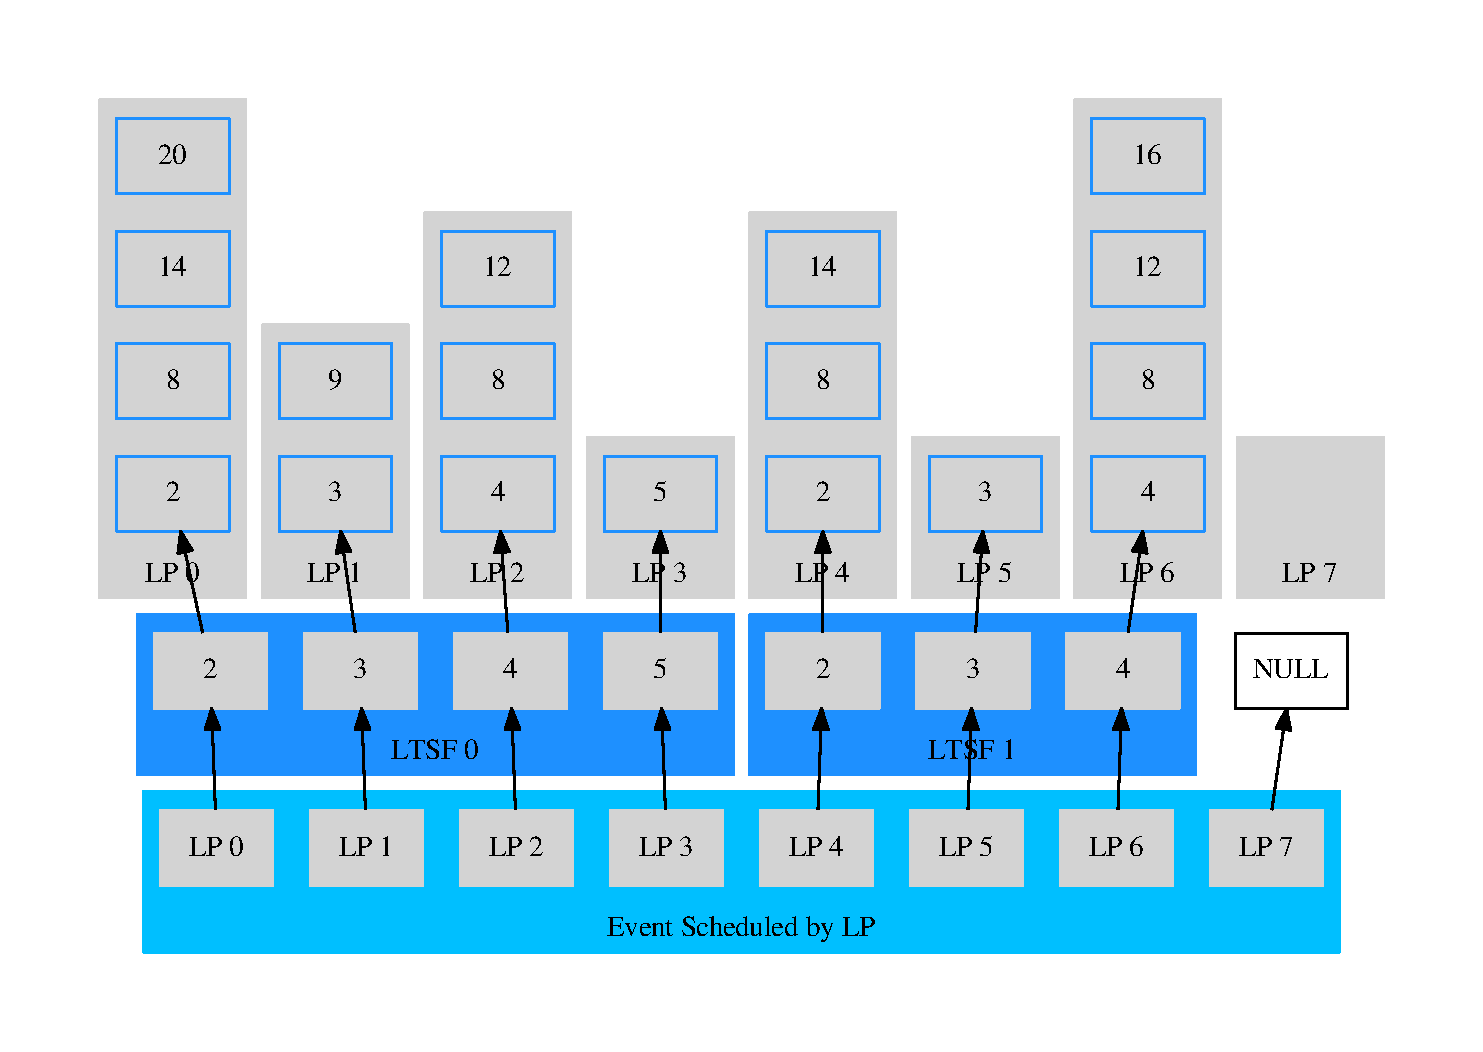
\includegraphics[width=0.75\textwidth]{figs/graphviz/pending_event_set.pdf}
    \caption{\textsc{warped2} Pending Event Set Data Structures}\label{pending_event_set}
\end{figure}

\section{Processing Events}

One or more of the worker threads are assigned to each LTSF Queue to process events from
and they all follow the exact same procedure. First, an event is removed from an LTSF
queue to be processed but remains in the unprocessed queue until it is completely processed or
cancelled out. The event is first checked against the last processed event of the receiving LP
to see if it is a straggler, and rolled back if necessary. An anti-message is also considered to
be a straggler if its positive counterpart was the last processed event for the LP since
\textsc{warped2} makes the assumption that message order will always be preserved.
So if the event is an anti-message, the positive counterpart is assumed to be in the LPs
unprocessed queue after rolling back and is cancelled out and a new event is scheduled into the
LTSF queue if another event is pending. If the event is positive then it is processed normally,
the state of the LP is saved, and new events are sent to other LPs. The event is then moved
into the processed queue and a new event is scheduled into the LTSF queue. To summarize the
worker thread processing loop is shown in psuedocode in algorithm \ref{warped2_processing}.

\begin{algorithm}
\DontPrintSemicolon
\SetKw{Continue}{continue}
\SetKwFunction{getNextEvent}{getNextEvent}
\SetAlgoVlined

    \While{termination not detected}{
        \nlset{1} $e \gets \getNextEvent{}$\;
        $lp \gets$ receiver of $e$\;\;

        \If{$e <$ last processed event for $lp$}{
            rollback $lp$\;
        }
        \;
        \If{$e$ is an anti-message}{
            cancel event with $e$\;
            \nlset{3} schedule new event for $lp$\;
            \Continue\;
        }
        \;
        process event $e$\;
        save state of $lp$\;
        \nlset{2} send new events\;
        \nlset{3} replace scheduled event for $lp$\;
    }

\caption{\textsc{warped2} Main Event Processing Loop}\label{warped2_processing}
\end{algorithm}

%% Sending events
When events are inserted into the unprocessed queues, they are compared to the currently
scheduled event for the LP. If there is no currently scheduled event or the new event is less
than the currently scheduled event, then the new event is scheduled to prevent a rollback from
occuring.

\subsection{Ordering of Events}

The time warp mechanism assumes that every event is labeled with a totally ordered clock value
based on virtual time \cite{jefferson-85}. This is important so that causal dependencies
are preserved and so that simulation results are deterministic\cite{ronngren-99}. To ensure
this, \textsc{warped2} uses a 4-tuple scheme which provide a total ordering of events:

\begin{enumerate}
    \item Receive Time
    \item Send Time
    \item Sender LP Name
    \item Generation
\end{enumerate}

\noindent %% tiebreaking
The last three serve as a tie breaker for simultaneous receive times. The send time is
necessary to ensure correct causal dependencies. It is analogous to a Lamport logical
clock\cite{lamport-78} in real time distributed systems but for virtual time systems. The
send time will work as long as LPs only send a single event with the same send time, receive
time, and receiver LP. Otherwise, a more strict ordering of sends would be required. However,
\textsc{warped2} forbids this behaviour in the simulation model. The sender LP name is necessary
to ensure that order is determined between events received with the same receive time and send
time from different senders. Without it, it is possible that different results could occur on
different runs of the simulation\cite{ronngren-99}. The generation is necessary for distributed
memory systems to differentiate between the same events which could be resent after rolling back
\cite{ronngren-99}. In \textsc{warped2} it is implemented as a single counter per LP and
keeps track of the number of events that have been sent from the LP. The count is then
tagged in the event when it is sent and used for comparison at the receiver.

\subsection{Performance Tuning Parameters}

To allow \textsc{warped2} to run on a large range of machines with different architectures and
characteristics, a number of parameters are provided for the user to tune the simulation mechanism
for their needs. In the current implementation, the four main parameters that will determine
performance are the number of worker threads, the number of LTSF Queues, the LTSF partitioning
method, and the state saving period.

\subsubsection{Worker Threads and LTSF Queues}

The number of worker threads that should be used will depend on the number of processors of the
machine so it is left as a tunable parameter. \textsc{warped2} also allows the user to choose
the number of LTSF queues. The user can specify any number of LTSF queues, however, it should
be smaller than the number of worker threads and also a factor. 

If all worker threads share a single LTSF queue then a huge contention point is created and
performance will suffer. At the opposite extreme, however, with all worker threads processing
events from a seperate LTSF queue, the the critical path of the simulation will be spread out
and the number of rollbacks can increase significantly. The extent to which these matter could
also vary as the data structures and algorithms evolve.

\subsection{LTSF Queue Partitioning}



\subsubsection{State Saving Period}

Instead of saving the state of the LPs after every processed event processed for them, \textsc{warped2}
allows the user to choose a state saving period value, $N$, so that each LP only has its state
saved every $N$ events. A larger the value of $N$ reduces the amount of time taken to copy states
and thus speeds up forward computation. The downside is that it also increases rollback time
since not all states are available to roll back to so more events will have to be processed to
get to the necessary state. The total time spent rolling back, however, is small compared to the
time taken for forward computation

\subsection{Protecting Access to LTSF Queues}

Worker threads must be able to access shared data structures without the possibility of
race conditions. To deal with this, \textsc{warped2} uses mutexes to serialize worker thread
access to any section of code that accesses the LTSF queue. This method, however can significantly
slows down access to the LTSF queues. In the default configuration, blocking mutexes are used
which means that if a thread cannot aqcuire a the lock, it will be put to sleep and rescheduled
for execution at a later time. However, this method can waiste a lot of exta time if access to the
critical section is quick. By looking back at figure \ref{warped2_processing}, we can see all
the critical points where worker threads can access the LTSF queues. The lines with a number on
the margin indicate possible access to the LTSF queue. For every event the LTSF queue is accessed
at least 3 times: \begin{inparaenum}[(1)] \item obtaining the next event, \item sending new
events, and \item rescheduling new events \end{inparaenum}. All of these accesses are quick so
the lock should only held for a short period of time.

A \emph{spinlock} is a type of mutex that does not force threads to be rescheduled but
instead continue to attempt to aqcuire the lock over and over until it successfully acquires
the lock or the timeslice of the thread expires. The downside of spinlocks is that the CPU time
can be waised, especially as the number of contending threads increase. Furthermore, if the
number of total threads is larger than the number of available processors, spinlocks are
even worse because a thread can be involuntarily pre-empted while holding the lock and entire
timeslices can be waisted.

\subsubsection{Spinlocks in \textsc{warped2}}

\textsc{warped2} allows the user to optionally build the kernel to use spinlocks instead of
blocking mutexes. It is not set as the default because spinlocks do not work well in all cases
such as with a system that is running more threads than processors.
There are many ways to implement spinlocks with all varying attributes and complexities.
Ticket locks were chosen for \textsc{warped2} because they are simple to implement, provide
fairness to all threads, and generally have good performance for a small number of threads
\cite{lockless-10}. A short psuedocode algorithm to illustrate the ticket lock aqcuisition and
release procedures is shown below in algorithm \ref{ticket_lock}.

\begin{algorithm}
\DontPrintSemicolon
\SetKwFunction{fetchAndIncrement}{fetchAndIncrement}
\SetKwBlock{Acquire}{lock}{end}
\SetKwBlock{Release}{unlock}{end}
\SetAlgoVlined

    \Acquire{
        $my\_number \gets \fetchAndIncrement{next\_number}$\;
        \Repeat{$ticket = my\_number$}{\tcp{do nothing}}
    }\;

    \Release{
        $\fetchAndIncrement{ticket}$
    }

    \caption{Ticket Lock Procedures}\cite{wiki:ticketlock-15}\label{ticket_lock}
\end{algorithm}

\noindent
To acquire the lock, each thread atomically increments a counter and takes the old value as
a "ticket" to provide first in first out order. Then when the ticket value reaches that
of the waiting thread, access to the critical section is given. To release the lock, the thread
simply increments the ticket number and allows the next thread to access the critical section.
If there is no contention for the lock, the next number will be equal to the ticket number and
a thread can access the critical section immediately.

\section{Data Structures to Support Rollback and Cancellation}

Jefferson\cite{jefferson-85} described the rollback and cancellation process in terms of three
data structures: the input queue, output queue, and state queue. The data structures that are
implemented in \textsc{warped2} follows pretty closely to Jefferson's description except that
in Jefferson's approach, the input queue holds both unprocessed and processed events whereas
\textsc{warped2} has two seperate data structures to allow easier scheduling of new events.

The state queues contain a 3-tuple value for each state. The first value is a pointer to a
memory location which holds the saved copy of the LP state. The second value is a pointer to the
event that produced the state of the LP and is used for comparison against a straggler event
on a rollback to determine which state to restore or against the GVT during fossil collection.
The third value is the state of the LPs random number generators at the time the state was saved.
The random number generator states are saved in a linked list and are also restored during a
rollback to ensure deterministic results.

Similar to the state queue, the output queue also contains a tuple of values. In the output
queue though, only a pointer to a source event and a sent events are used. In the same way
as the state queue, the source event is used for comparison against a straggler event during
a rollback but is used to determine which events should be sent as anti-messages.

The processed queues only contain a pointer to the processed events. The dereferenced events
from the processed queue are the same as dereferenced source events from output queue and state
queue so that no copying of the events is needed. Furthermore, if events are sent withing the
same process, the same events can be pointed to from the output queue and an unprocessed or
processed event from another LP. The organization of the processed queue, state queue and output
queue for a single LP is illustrated in figure \ref{rollback_ds}.

\begin{figure}[H]
    \centering
    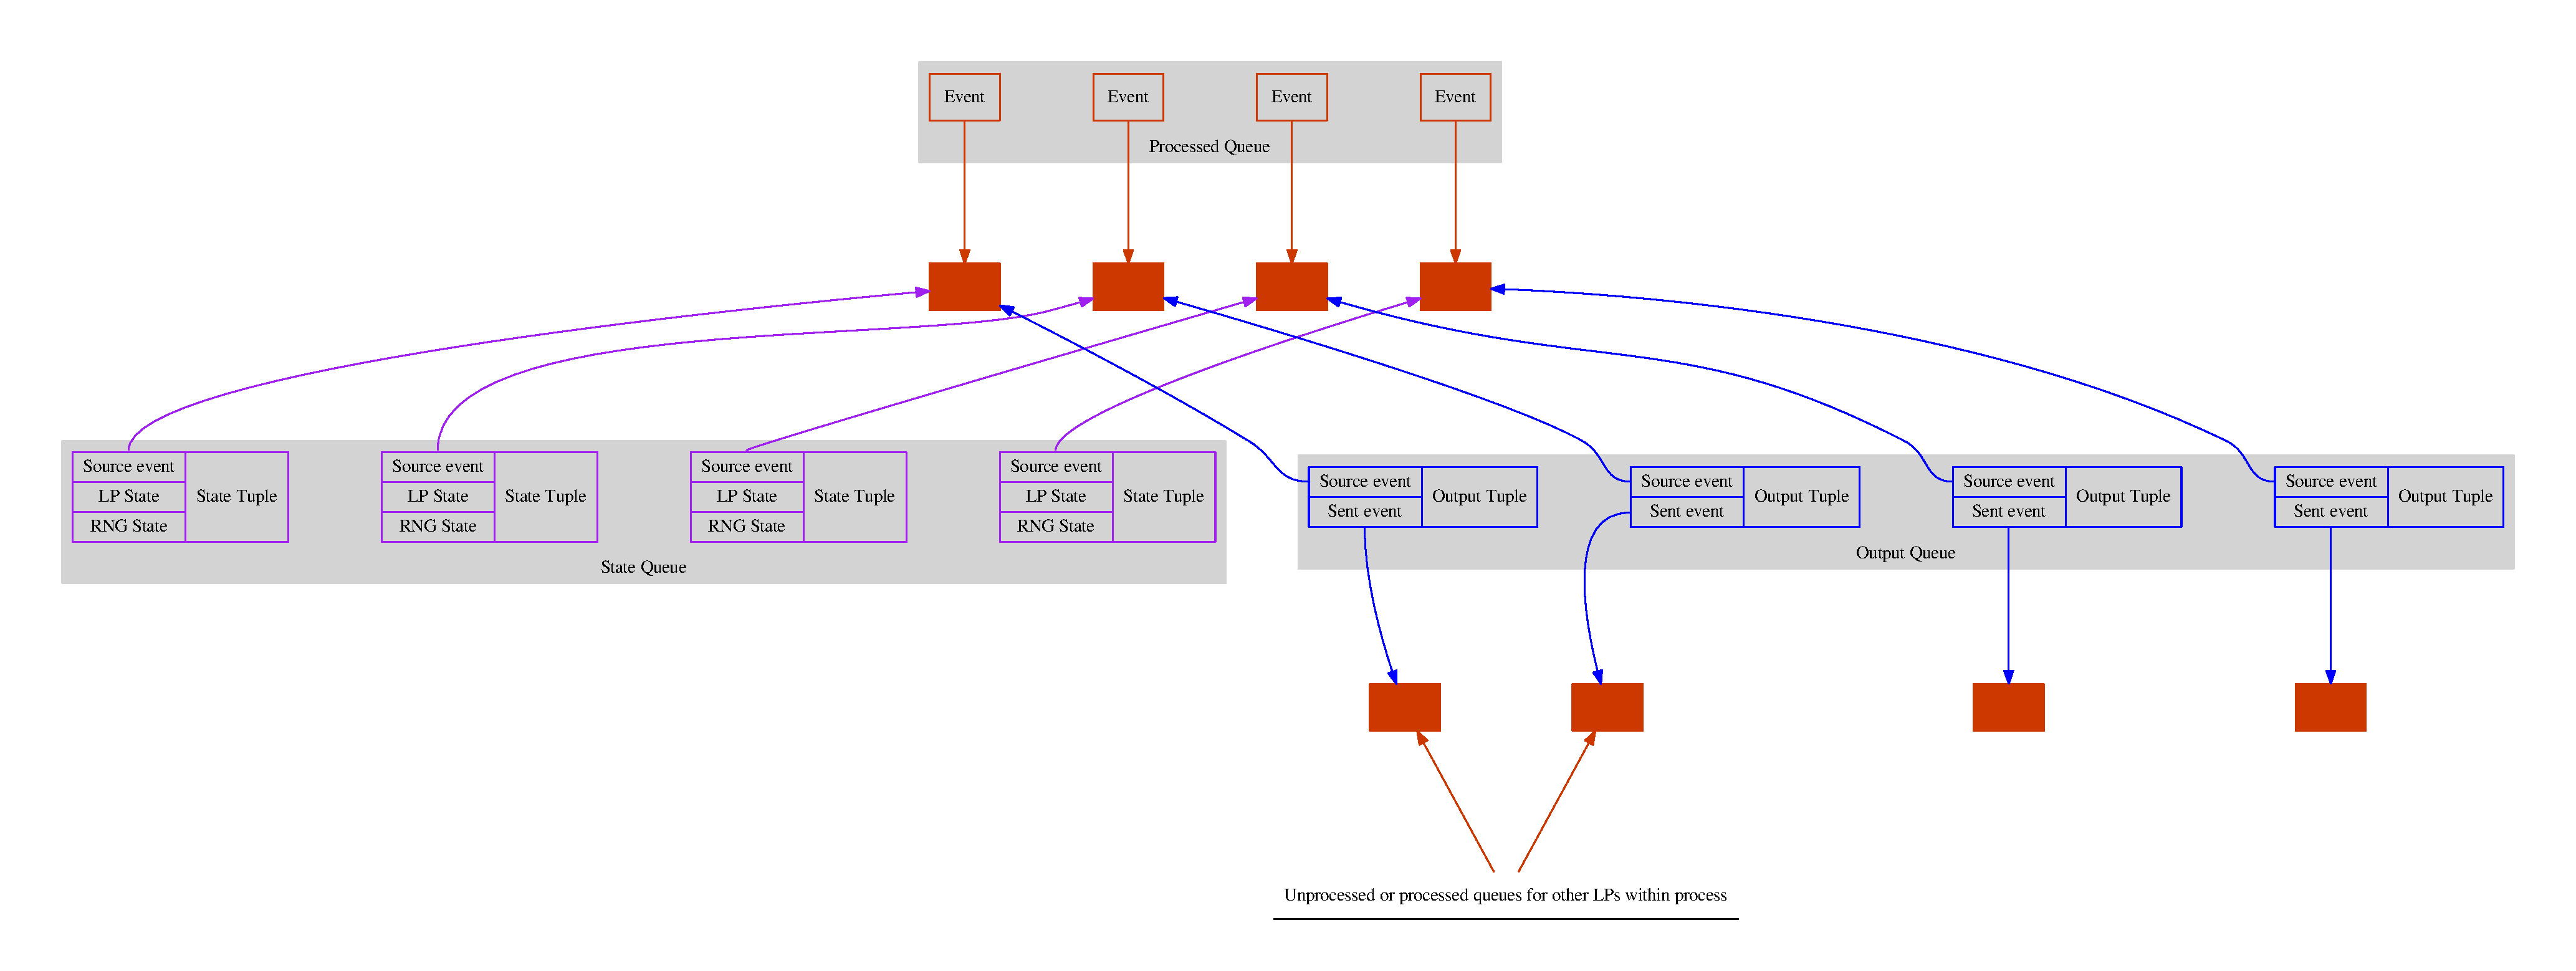
\includegraphics[width=\textwidth]{figs/graphviz/rollback_ds.pdf}
    \caption{Rollback and Cancellation Data Structures in \textsc{warped2}}\label{rollback_ds}
\end{figure}

Although the organization of these data structures prevents copying of events, there are also
some limitations. First, it introduces a lot of indirect memory accesses which could slow down
access to memory, especially in a multiprocessor system. Secondly, it adds some complexity
when freeing memory used by events. To solve this problem though, \textsc{warped2} uses the
smart pointers offered by the standard C++11 libraries which employ a reference counting
scheme.



\chapter{GVT and Termination Detection}\label{gvt_termination}

Algorithms that compute the Global Virtual Time (GVT) and detect termination conditions are
both examples of algorithms that can be solved by determining the global state of a
distributed system. The global state of a system is defined as the combination of all
the local states of the processes in the system and all messages in transit. Global state
determination algorithms are also commonly used for deadlock detection, garbage collection,
debugging, and checkpointing for failure recovery in distributed systems.

\section{Global Snapshots}

\paragraph{Chandy and Lamport}\cite{chandy-85} described a basic global state algorithm by
using \emph{global snapshots} for distribtuted systems that use only FIFO channels for
communication. To start the algorithm, an initiator process records it's state and sends
a control token out of all outgoing channels. When a process receives a control token, and
it hasn't yet recorded its state, the process records its state and sends more control
tokens out of all its outgoing channels. The algorithm terminates at each process when it
has recieved a token through all of its incoming channels.

\paragraph{Lai and Yang}\cite{lai-87} describe an algorithm for non-FIFO systems which
computes a consistent cut by piggybacking a control bit onto basic messages. The control
bit is used to indicate whether or not the sending process has recorded its state. The
processes can be explained in terms of colors. A process that has not recorded its state
is colored white and a process that has recorded its state is red. White processes send
white messages and red processes send red messages. The control bit in the messages indicates
the color. All processes are initially white and turn red when a red message arrives. When
a red message arrives at a white process, the process must record its state BEFORE actually
receiving the message. The snapshot only relies on basic messages and no control tokens are
used. This algorithm has several drawbacks. First, it assumes that every process will
eventually receive a red message and record its state which is not guarenteed. Second, to
ensure transient messages are recorded, the processes must record all incoming and outgoing
messages and send them to other processes within the basic messages. That way the transient
messages can be calculated by differences in incoming and outgoing messages.

\paragraph{Mattern}\cite{mattern-93} extended the algorithm by Lai and Yang by adding a
seperate control token which is used to create two cuts by cirulating the control token to
every process twice. The control token is used to color the processes instead of the basic
messages. This guarentees that every process will eventually record its state because the
token is always circulated. Furthermore, processes do not have to keep track of sent and
received messages. Instead counters can be used to keep track of the differences in sent
and received white messages at each process. The control token can then accumulate the
counts. When the white message counts accumulate to zero when the token arrives back at
the initiator proccess, it can be determined that the snapshot is complete. These counters
can be \emph{vector counters} or \emph{scalar counters}. Vector counters keep track of
messages to/from each process individually whereas scalar counters keep track of just a
single count at each process. When the algorithm is complete, only the initiator process
can produce a global snapshot so if all processes must use the snapshot, it must be broadcasted
to the other processes.

\section{GVT}

Although GVT algorithms can be implemented with the basic global snapshot algorithms described
above, it is usually more efficient to build custom solutions on top of the basic algorithms.
In a GVT algorithm, the local minimum clock of process is the local state and the basic
messages are events that are sent between processes. This section first describes the key
ideas that must be considered when developing a GVT algorithm. Then, a few of the classic
GVT algorithms and modern GVT algorithms that are commonly used in practice today are described.
Finally, the algorithm that is implemented in \textsc{warped2} is described as well as the
reasons for choosing the approach.

GVT algorithms can be synchronous or asynchronous. In a synchronous GVT algorithm, since
all other computation will be blocked, event processing will be halted. Synchronous GVT
algorithms are usually very simple to implement but halting the event processing can
be very costly. On the other hand, asynchronous GVT algorithms calculate GVT concurrently
with event processing. For this reason, asynchronous GVT algorithms perform much better
than synchronous GVT algorithms but are harder to implement because special cases must be
considered.

There are two special cases that must be considered in any GVT algorithms:

\begin{description}
    \item[Transient Message Problem:] is caused by messages(events) that have been sent by
    the sending process but not yet recieved by the receiving process. If not carefully
    considered in a GVT algorithm, these \emph{transient messages} can be completely missed
    which could lead to an erroneous GVT calculation if they contain the minimum timestamp
    of all other events in the system.
    \item[Simultaneous Reporting Problem:] is caused because processes can report their local
    minimum clock at different points in real time. Consideration must be taken into account
    to ensure that a process does not report its local minimum clock value and then receive
    an event from a process that has not yet reported its local minimum clock value,
    completely missing the event.
\end{description}

\noindent
There are many synchronous and asynchronous GVT algorithms that have been developed over the
years that all have some method of either solving these problems.

\subsection{Asynchronous GVT Algorithms}

\subsubsection{Message Passing Algorithms}

Most of the time warp systems in use today are based on message passing and classically
GVT algorithms have been designed for message passing systems. In this section Samadi's and
Mattern's message passing algorithms are discussed and in the next section Fujimoto's shared
memory GVT algorithms is discussed as well as the Seven O'Clock algorithm which is an
extension of Fujimoto's shared memory algorithm extended for distributed memory systems.

\paragraph{Samadi's Algorithm}\cite{samadi-85} in the most general form uses acknowledgements
for all events that have been received. All processes must track all events that have been
sent but have not been acknowledged. Furthermore, the received messages must also be tracked
so that acknowlegements can be sent. All transient message can then be calculated from the
tracked messages. A process initiates the GVT algorithm by broadcasting a start message to
all processes. After this start message is received by a process, it is marked(colored) and
all acknowledgements sent from a marked process are also marked(colored). All processes then
calculate their local minimum by taking the minimum of the unacknowledged received events,
the marked acknowledgments sent, and the local simulation clock. Marking the acknowledgements
sent after the start of the GVT calculation ensures that the simultaneous reporting problem
will not occur.

\paragraph{Mattern's Algorithm}\cite{mattern-93} for GVT calculation is an extension on his
general snapshot algorithm that was described above. The white message counts are used to
determine whether transient messages are still in the sytem. They also serve as the basis
for determining when the snapshot is complete which occurs when the accumulated white message
count of all processes is zero. To ensure that the simultaneous reporting problem does not
occur, red messages received at a white process are recorded and used in the local minimum
value. The algorithm is initiated by sending a control token to all processes in some defined
order. The token accumulates the white message counters, local minimum clocks, and minimum
red message timestamps. When the accumulated count reaches zero and the token is back at
the initiator process, the GVT is approximated using the minimum of the accumulated clocks
and timestamps.

\paragraph{Other GVT Algorithms} that are based on message passing model are usually based
on the same ideas from Samadi's algorithm or Mattern's algorithm. Many algorithms are just
extensions or variations of the algorithms that aim to optimize it in some particular way.

\subsubsection{Shared Memory Algorithms}

\paragraph{Fujimoto's Algorithm}\cite{fujimoto-94} is a fast GVT algorithm that exploits
properties of shared memory architectures. In most shared memory architectures, processors
cannot observe memory operations in different orders. For this reason, it is not possible
to have transient messages if a shared data structure is used to communicate between tasks
running on different processors. Furthermore, a shared flag variable can be used to initiate
the GVT algorithm. However, it is still possible that the flag can be read at different
times, so the simultaneous reporting problem can still occur. To solve the simultaneous
reporting problem, two things must be done, First, the start flag is checked after sending
events and recorded if the sending task has not yet reported its local minimum value and
is eventually used when the reporting is done. Second, the start flag must be read into a
temporary local variable before obtaining a new event to process.

\paragraph{Seven O'Clock Algorithm}\cite{bauer-05} is an extension of Fujimoto's algorithm
for distributed memory systems. Although the algorithm can be used in message passing systems,
the algorithm does not use any messages and is still uses shared memory ideas. The key idea
in the algorithm is that all processors in a distributed system all have a consistent view
of wall clock. Hence, the processors can carry out an operation atomically, without having
to explicitly interact. The atomicity can be achieved by using cycle level counters which
are available on most modern architectures. Unlike Fujimoto's algorithm though, transient
messages can still be missed in the calculation. To solve that problem, each processor must
wait a small time interval which is calculated based on the worst round trip time for
network transactions.

\subsection{Synchronous GVT Algorithms}

\paragraph{Global Reductions} provide a good way to do a synchronous minimum calculation
which and is a common way to implement a synchronous GVT algorithm. ROSS implements a
synchronous GVT algorithm which uses global reductions\cite{holder-08}. First, to prevent
the transient message problem, a global reduction on message counts of each process is
performed until it reaches zero which is guarenteed because the reduction acts as a barrier
for each process. The message counting is necessary because asynchronous communication is
used for sending and receiving events. When the messages count reaches zero a global
reduction is performed on the local minimum timestamp of all processes to give a GVT value
which is broadcast to all processes. This algorithm is efficient when time warp simulation
are run on large supercomputing platforms like the blue gene machine which perform collective
operations very quickly.

\subsection{GVT in \textsc{Warped2}}

To calculate the GVT in \textsc{warped2}, Fujimoto's shared memory algorithm is used between
worker threads and a variation of Mattern's algorithm with scalar message counters is used
between processes. Fujimoto's algorithm is a subalgorithm of Mattern's algorithm. The details
of the Mattern's algorithm implementation in \textsc{warped2} is detailed below as well as how
it is used with Fujimoto's algorithm. More details on Fujimoto's algorithm will not be detailed
but they can be found by reading \cite{fujimoto-94}.

In the \textsc{warped2} implementation, scalar counters are used to keep track of message
that are sent that carry the initial color. That means that each process keeps track of
the number of sent messages minus the number of received messages to and from all other
process as a single count. The reason that scalar counters are used over vector counters
is that vector counters require that communication is stopped after receiving a control token
until all known transient messages that are bound for the receiving process are received. With
scalar counters, this is not possible because all counts are combined into a single counter.
However, with scalar counters it is possible that more than two rounds of the control token will
be necessary. This is usually not a problem in practice though since two rounds is usually
sufficient. Also, each process must maintain a counter for both white messages \emph{and} red
messages so that counters can be consistent between multiple runs of the algorithm. The roles of
the colors must also be switched between successive runs.

In the description of the \textsc{warped2} algorithm, the colors will be described as
\emph{initial} and \emph{final}, where the \emph{initial} color is the starting color for each
process before receiving a token and the \emph{final} color is the color after receiving the
token. Each process keeps track of its current color, a minimum timestamp of an event received
with the final color, and temporary variables to hold accumulated values from the token. The
variables that will be used in the following discussion are listed below in algorithm
\ref{process_variables}.

\begin{algorithm}
\DontPrintSemicolon
    \boldmath$ts_{min}:$ Minimum timestamp of event messages received with final color\;
    \boldmath$color:$ Current color of the process\;
    \boldmath$color_{initial}:$ Intial color of all processes\;
    \boldmath$msgcount_{initial}:$ Messages sent minus messages received with initial color\;
    \boldmath$msgcount_{final}:$ Messages sent minus messages received with final color\;
    \boldmath$clock_{min}:$ Temporary variable to hold accumulated minimum clock from all processes\;
    \boldmath$msgcount:$ Temporary variable to hold accumulated initial color message count
        from all processes\;
\caption{Process Variables in \textsc{warped2} Mattern Implementation}\label{process_variables}
\end{algorithm}

\noindent
The event messages that are sent between processes have the format:

    $<sender, receiver, mcolor,...>$

\noindent
where $sender$ is the id of the sender process, $receiver$ is the id of the reciever process,
and $mcolor$ is the color of the message. The message color is the color of the sending
process at the time it is sent. The message count for the current color is also incremented
when it is sent. The event sending procedure is shown below in algorithm \ref{gvt_event_send}.

\begin{algorithm}
\DontPrintSemicolon
\SetAlgoVlined
    $mcolor \gets color$\;
    \If {$color = color_{initial}$} {
      $msgcount_{initial} \gets msgcount_{initial} + 1$\;
    }
    \Else {
      $msgcount_{final} \gets msgcount_{final} + 1$\;
    }
\caption{Event Message Send}\label{gvt_event_send}
\end{algorithm}

When an event is received by a process, the message count for the current color of the process
is decremented. If the color carried by the message is the final color indicating that the
sender has already reported a local minimum value, then the timestamp of the event is recorded.
The procedure for receiving an event is shown below in algorithm \ref{gvt_event_receive}.

\begin{algorithm}
\DontPrintSemicolon
\SetAlgoVlined
    \If{$color_{message} = color_{initial}$} {
        $msgcount_{initial} \gets msgcount_{initial} - 1$\;
    }
    \Else {
        $msgcount_{final} \gets msgcount_{final} - 1$\;
        $ts_{min} \gets \min{(ts_{min}, ts_{event})}$\;
    }
\caption{Event Message Receive}\label{gvt_event_receive}
\end{algorithm}

\noindent
The control token that is sent between processes has the format:

    $<sender, receiver, mclock, msend, mcount>$

\noindent
where $mclock$ is an accumulated minimum of all local minimum clocks at all processes
visited by the token, $msend$ is an accumulated minimum of all $ts_{min}$ values at all
processes visited by the token, and $mcount$ is an accumulated sum of the final message count
($msgcount_{final}$) from all processes visited by the token.

The token is passed in logical ring fashion to increasing process ids and is initiated by process
with id 0. When the token reaches process $N-1$, where $N$ is the number of processes, it is
sent back to process 0. To start the algorithm, the initiating process toggles its color, resets
minim values to infinity, stores the initial color message count into a temporary variable
($msgcount$), and starts Fujimoto's algorithm. When Fujimoto's algorithm is complete, it will
send the token $<0, 1, lvt_{min}, ts_{min}, msgcount>$ with $lvt_{min}$ being the result of
Fujimoto's algorithm. The start procedure is illustrated below in algorithm \ref{gvt_start}.

\begin{algorithm}
\DontPrintSemicolon
\SetAlgoVlined
\SetKwFunction{SendToken}{SendToken}
\SetKwFunction{Fujimoto}{doFujimoto}
    \If{$color = WHITE$}{
        $color \gets RED$\;
    } \Else {
        $color \gets WHITE$\;
    }
    $ts_{min} \gets \infty$\;
    $clock_{min} \gets \infty$
    $msgcount \gets msgcount_{initial}$\;
    $msgcount_{initial} \gets 0$\;
    $lvt_{min} \gets \Fujimoto{}$\;
    \SendToken{$0, 1, lvt_{min}, ts_{min}, msgcount$}\;
\caption{Mattern Algorithm Start Procedure}\label{gvt_start}
\end{algorithm}

When a token is received at a process that is not the initiator and it still has the initial
color then the color is toggled. Then, the minimum timestamp received from final colored
messages, the minimum clock value, and the initial message count for the process are
accumulated with the token's values. The initial message count is then reset so it will not
be used in the next round and Fujimoto's algorithm is initiated. When Fujimoto's algorithm
is completed, the token is sent to the next process with all of the accumulated values
including $lvt_{min}$ calculated from Fujimoto's algorithm. The token receive procedure for
non-initiator processes is illustrated below in algorithm \ref{gvt_receive_noninit}.

\begin{algorithm}
\DontPrintSemicolon
\SetAlgoVlined
\SetKwFunction{SendToken}{SendToken}
\SetKwFunction{Fujimoto}{doFujimoto}
    \If{$color = color_{initial}$} {
        $ts_{min} \gets \infty$\;
        \If{$color = WHITE$}{
            $color \gets RED$\;
        } \Else {
            $color \gets WHITE$\;
        }
    }
    $ts_{min} \gets \min{(ts_{min}, msend)}$\;
    $clock_{min} \gets \min{(clock_{min}, mclock)}$\;
    $msgcount \gets msgcount_{initial} + msgcount$\;
    $msgcount_{initial} \gets 0$\;
    $lvt_{min} \gets \Fujimoto$\;
    \SendToken{$i, (i+1) \bmod N, \min{(lvt_{min}, clock_{min})}, ts_{min}, msgcount$}\;
\caption{Mattern Control Token Receive Procedure: Non-initiator Node}\label{gvt_receive_noninit}
\end{algorithm}

When a token is received at a the initiator process, it can be assumed that a minimum clock
value has already been included in the token that is received. If the accumulated message count
for the initial color has reached zero, then the GVT can be appoximated and the algorithm
is terminated. If there are still transient message that were not accounted for, the initiator
process initiates a new round until the resulting message count accumulation is zero
when received at the initiator. The GVT is approximated at the initiator by taking the
minimum of the accumulated minimum clock values and the accumulated minimum timestamp values.
The estimated GVT value is then broadcast to the rest of the processes. The token receiving procedure
for the initiator process is illustrated below in algorithm \ref{gvt_receive_init}.

\begin{algorithm}
\DontPrintSemicolon
\SetAlgoVlined
\SetKwFunction{SendToken}{SendToken}
\SetKwFunction{Fujimoto}{doFujimoto}
\SetKwFunction{SendGVTUpdate}{SendGVTUpdate}
    \If {$mcount = 0$} {
        $gvtApprox \gets \min{(mclock, msend)}$\;
        \SendGVTUpdate{}\;
        \If{$color_{initial} = WHITE$}{
            $color_{initial} \gets RED$\;
        } \Else {
            $color_{initial} \gets WHITE$\;
        }
        $clock_{min} \gets \infty$\;
    } \Else {
        $ts_{min} \gets \min{(ts_{min}, msend)}$\;
        $msgcount \gets msgcount_{initial} + mcount$\;
        $msgcount_{initial} \gets 0$\;
        $lvt_{min} \gets \Fujimoto$\;
        \SendToken{$i, (i+1) \bmod N, lvt_{min}, ts_{min}, msgcount$}\;
    }
\caption{Mattern Control Token Receive Procedure: Initiator Node}\label{gvt_receive_init}
\end{algorithm}

\section{Termination Detection}

Termination detection, like GVT, is a problem of determining the global state of the system.
Termination is a \emph{stable property} of a distributed system, meaning that once termination
conditions occur, the system will remain with termination conditions forever until further
action is taken.

A process in the system can be in one of two states at any time: active or passive. A process
is considered active if some basic computation still remains and passive otherwise.
When all processes in the system become passive and no messages are left in transit, then
the system should be terminated. The purpose of the termination detection algorithm is to
determine when this occurs. A passive process can become active with the arrival of an
\emph{activation message}. For parallel discrete event simulation the basic computation is
event processing and the activation messages are events. A termination detection algorithm for
any parallel discrete event simulation must satisfy the following properties:

\begin{description}
    \item[Safety Property:] Termination will not be detected if any unprocessed event is still
        present in system which includes all local pending event sets and events still in transit.
    \item[Liveness Property:] Termination will be detected at some finite amount of time after
        all events have been processed.
\end{description}

Just like GVT algorithms, termination detection algorithms can implemented with message
passing or shared memory communication. Termination algorithms vary widely because different
systems can define termination conditions in such different ways. Furthermore, termination
usually does not affect system performance as long it does not block event processing so
correctness is more important than optimization. The rest of this section will only focus
on the algorithms that are implemented in \textsc{warped2}.

\subsection{Termination in \textsc{warped2}}

The termination detection algorithm in \textsc{warped2} is actually two independant algorithms,
a message passing algorithm and a shared memory algorithm. In the opposite manner as the
GVT algorithm, the shared memory algorithm is actually used to initiate the message passing
algorithm.

\subsubsection{Shared Memory algorithm}

The purpose of the shared memory algorithm is to determine when all of the worker threads
in a process become passive (inactive). The algorithm is fairly straightforward and uses
just a shared counter variable to keep track of the number of active worker threads and a
boolean array to keep track of which worker threads are active. Worker threads update their own
state when they change and atomically update the counter. The manager thread periodically
checks to see if the counter has reached zero. If the count has reached zero and the process
is the master, then the interprocess message passing alorithm is initiated.

The safety property is not necessarily achieved because it is possible that the last active
thread sends an event to another LP which will be processed by another thread. Then if the sending
thread becomes inactive, all threads can be temporarily inactive and the manager thread can
falsely detect termination. However, it is very unlikely that the sending thread will report
itself as passive before the receiving thread gets the event and reports itself as active.
Furthermore, the manager thread is forced to check the active thread counter at least twice with
no changes in any worker thread state. The liveness property is achieved because the manager
thread periodically checks the active worker thread count so the inactivity of all worker threads
will eventually be discovered.

\subsubsection{Message Passing Algorithm}

The algorithm that is carried out among processes is an asynchronous message passing
algorithm based on Mattern's "sticky flags" algorithm\cite{mattern-93}. Just like the GVT
algorithm, the token is passed in a logical ring to increasing process ids. However, the
initiator process of the algorithm is dynamic. The initiator is the first active process
that the token reaches during circulation. For the first circulation, the initator is process
0.

Each process has two states, one for the actual state and one for the \emph{sticky state}.
The sticky state is the state that is actually used in the algorithm. It becomes active
when the actual state becomes active but sticks to active when the actual state becomes
passive. The sticky state can only changes to passive on the arrival of a token. By using
this scheme the token is forced to circulate two times with no process becoming active and
ensures the safety property. Without this scheme, a process that has already forwarded the
token because it was passive could receive an activation message and then the sender of the
activation message could become passive before receiving the token. False termination could
then be detected.

The process variable names that are used for the succeeding discussion are listed in
algorithm \ref{termination_variables}.

\begin{algorithm}
\DontPrintSemicolon
    \boldmath$state_{actual}:$ Indicates the actual state of the process at all times\;
    \boldmath$state_{sticky}:$ Indicates the state of the process if active, but may stick
        to active if passive\;
    \boldmath$initiator:$ Boolean variable indicating process is leader\;
\caption{Process Variables in Termination Detection Algorithm}\label{termination_variables}
\end{algorithm}

\noindent
The termination token that is sent between process has the format:

    $<sender, receiver, mstate, minitiator>$

\noindent
where $sender$ is the id of the sending process, $receiver$ is the id of the receiving
process, $mstate$ is the partial state of system based on visited processes, and $minitiator$
is the process id of the initiator.

The algorithm is started when the initiator process becomes passive which is determined by
the shared memory algorithm. When a process receives the token it becomes the initiator
but loses its roles as initiator when it sends the token. That way, only a single process
can be the initiator. Furthermoe, since the token always stops at an active process, the
token is always guarenteed to start again when it becomes passive which also guarentees
the liveness property. When the token is received back at the initiator with a passive
state, then termination is signaled to all processes. The procedure is illustrated in
algorithm \ref{termination_token_receive}.

\begin{algorithm}
\DontPrintSemicolon
\SetAlgoVlined
\SetKw{And}{ and }
\SetKwFunction{SendToken}{SendToken}
    $initiator \gets true$\;
    \If{$state_{sticky} = PASSIVE \And state_{process} = minitiator$} {
        \If{$mstate = PASSIVE$} {
            Signal termination\;
        }
    } \ElseIf{$state_{sticky} = PASSIVE$} {
        $initiator \gets false$\;
        \SendToken{$mstate, minitiator$}\;
    }
    $state_{sticky} \gets state_{actual}$\;
\caption{Termination Token Receive Procedure}\label{termination_token_receive}
\end{algorithm}

It should also be noted that this algorithm is only guarenteed to work if the message order
is preserved. If that is not the case, then message counters are necessary to ensure
transient activation messages are not missed.



\chapter{Memory Management}\label{memory_management}

This chapter will focus on main topics related to memory management in a time warp system
and their implementations in \textsc{warped2}. The topics will include state saving, fossil
collection and memory allocation. Different methods for each of these topics have different
time and memory requirements and vary greatly in complexity.

\section{State Saving}

\subsection{State Saving Techniques}

\paragraph{Copy-state Saving} is the classic state saving technique that saves every past
state of every LP and requires that the all states are copied and saved into the state queues.
This method requires a lot of extra memory and requires a lot of extra computation to copy
the states and insert them into the state queue. For this reason, copy-state saving is
usually used in conjuction with other technique or not at all.

\paragraph{Periodic State Saving} is another state saving technique where the state of each LP
is saved only once every N events, where N is a number greater than one. Periodic state
saving can significantly reduce the overhead of the time taken to copy the state of the
LPs into the state queue. However, due to state history being lost, more processed event
have to be saved so that the state of LPs can be restored correctly. These saved events
must be reprocessed to restore the state in a process known as \emph{coast forwarding}.
During coast forwarding the events are processed normally but only to update the state.
The only difference is that no events are sent during the coast forwarding phase. The
downside is that the rollback length is increased due to the loss in state saving. However,
periodic state saving is a significant improvement over the base copy-state staving approach
since the reduced time in state saving far outweighs the extra rollback time for increased
rollback length.

\paragraph{Incremental State Saving} is a technique that aims to reduce the amount of
memory needed to store past states of the LPs. Instead of saving entire snapshots of the
past states, the differences in specific state variables are saved. This method requires
that metadata describing which variables are modified for each event. Therefore, this approach
works well as long as only a small portion of the state variables change during the forward
execution of events.

\paragraph{Reverse Computation} is a modern approach to state state saving that does not
actually save any past states of the LPs. Instead, the \emph{control state} of the forward
computation is saved as a set of bits that describe the control flow. By saving the control
flow of the forward execution for each event, the state variables that are modified and
how they are modified are known and can be reversed. That is, at least, if all state variables
are reversible without the need to know the histories of the variables. Also, a reversible
random number generator is required. These are both practical requirements, though. The major
problem with this approach is the necessity to understand forward and reverse computation
precisely in the implementation of the simulation model.

\subsection{State Saving in \textsc{warped2}}



\section{Fossil Collection}

When the events and states in the processed queues, output queues, and state queues are
no longer needed, the memory that they consume is no longer needed and can either be freed
or reused. Fossil collection is the process of reclaiming memory for future use. There
are many methods of fossil collection that have been used in practice.

\subsection{Fossil Collection Techniques}

\paragraph{GVT-based Fossil Collection} is the traditional method of fossil collection.
Since rollbacks cannot occur past the GVT, it can be used be used as a marker to indicate
what can be fossil collected. In this case, the calculation of the GVT generally triggers
the fossil collection process and all memory is explicitly freed so that it can be reused
again.

\paragraph{On-the-fly Fossil Collection} is a method of fossil collection used in GTW
which does not use GVT and memory is not explicitly freed. Instead, after events are
processed, they are added to a free memory list. New events can then be allocated from the
list as long the first event in the list has a timestamp less than the GVT. If it does not
then the current event being processed is either aborted until the GVT reaches a higher
value or the list is searched for a lower timestamp event.

\paragraph{Optimistic Fossil Collection} is another method of fossil collection which
aims to reuse memory instead of explicitly freeing it. However, optimistic fossil collection
is based on a statistical bound for rollbacks. It is still possible that memory that was
fossil collected could still be used causing an OFC fault. Therefore, methods such as
global state checkpointing must also be implemented to recover from these faults.

\subsection{Fossil Collection in \textsc{warped2}}



\section{Memory Allocation}

Parallel discrete event simulation systems must frequently allocate and free memory for
events and states. This can be a huge overhead if used memory and free memory is not
maintained in an efficient way. Furthermore, memory must be allocated to and deallocated from
each process by the operating system as needed which can be even more costly.

In a standard system, the application will never know when memory is allocated from the operating
system or returned to it because it is usually handled by runtime libraries for the programming
language that is used which provide an API for allocation/deallocation for each specific
process. To completely remove an OS overheads, some time warp systems allocate a large fixed
sized memory space before the start of the simulation and use their own memory management
schemes. In these time warp systems, the simulation kernel must provide a way for the simulation
models to allocate memory for events that need to be sent instead of calling the standard programming
language APIs.

Dynamic memory management in \textsc{warped2} is achieved through the standard malloc/free
interface just like any other C/C++ application and does not pre-allocate any memory. The
simulation model is responsible for the allocation of all states and events. The kernel only
receives pointers to the states and events and accesses them indirectly. By doing this, we
allow simulation model developers to implement their own memory management schemes or override
the default malloc with allocators such as TCMalloc, JEMalloc, Hoard, etc.


\section{Memory Tuning Parameters in \textsc{warped2}}



\subsection{State Saving Period}



\subsection{GVT Period}





\chapter{Experimental Analysis}\label{experimental_analysis}

This chapter will focus on analyzing the behavior of \textsc{warped2} to find the best parameters
to fine tune the simulations for best performance. The focus will be on single x86 SMP nodes
and x86 clusters for now and in chapter \ref{big_little_platform}, some experiments will be
run on ARM nodes.

\section{x86 SMP Nodes and Cluster}

Experiments with x86 platforms will consist of a set of experiments targeted at a single node
SMP processor and a set of experiments targeted at a beowulf cluster. The goal for all x86
experiments will be to figure out how to configure the \textsc{warped2} simulation kernel for
the best performance while keeping memory requirements and stability in mind.

The single node SMP experiments will be run on an Intel Xeon X5675 processor. The intel X5675
has 6 cores with hyperthreading so that 12 simultaneous threads are supported.
Cluster experiments will be run on Intel Xeon E5410. The Intel Xeon E5410 is a quad core processor
but our system contains two sockets per machine so that 8 cores per machine are available.
A summary of the architectural features of both machines that used are shown in table
\ref{x86_platform}.

\pagebreak

\begin{table}
    \centering
    \begin{tabular}{|| l | l | c | c ||}
    \hline
    & & Intel\textsuperscript{\textregistered} Xeon\textsuperscript{\textregistered} X5675 &
        Intel\textsuperscript{\textregistered} Xeon\textsuperscript{\textregistered} E5410 \\ [0.5ex]
        \hline\hline
        \multirow{8}{*}{Processor}
            & ISA           & x86\_64   & x86\_64   \\
            & \# Cores      & 6         & 8         \\
            & \# Threads    & 12        & 8         \\
            & \# Sockets    & 1         & 2         \\
            & Frequency     & 3.06 GHz  & 2.33 GHz  \\
            & L1 Data Cache & 32kB      & 32kB      \\
            & L1 Inst Cache & 32kB      & 32kB      \\
            & L2 Cache      & 256kB     & 6MB       \\
            & L3 Cache      & 12MB      & N/A       \\
        \hline
        \multirow{3}{*}{Runtime}
            & Compiler      & GCC v4.9.2 & ? \\
            & MPI Version   & MPICH v3.1 & ? \\
            & Malloc        & TCMalloc v2.4 & \\
        \hline
    \end{tabular}
    \caption{x86 Assessment Platforms}\label{x86_platform}
\end{table}

\section{Simulation Models}

\subsection{PCS}

The model describes a type of wireless communication network known as a Portable Cellular
Service (PCS) network. A PCS network provides services for a number of \emph{portables} which
are the subscribers to the network. The service area of the network is divided into
\emph{cells} and a single \emph{port} covers a cell which has a certain number channels that
it can allocate for calls. When an incoming or outgoing call is made, a port must allocate
a channel from the port if one cannot be allocated then the call is \emph{blocked}\cite{lin-96b}.
The only type of logical processes in the PCS simulation are the cells. The cells in the
\textsc{warped2} model form a rectangular grid as shown in figure \ref{pcs_model_lps}.
Portables can only move to other cells from an adjacent cell with a wrap around occuring
at the edges.

\begin{figure}[H]
    \centering
    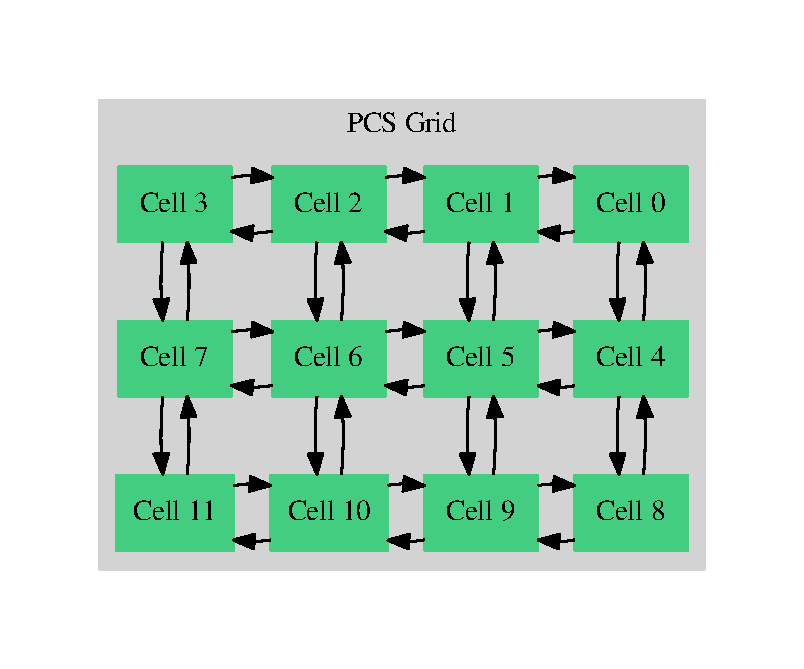
\includegraphics[width=0.6\textwidth]{figs/graphviz/pcs_model.pdf}
    \caption{PCS Model Logical Processes}\label{pcs_model_lps}
\end{figure}

The portables stay within a cell for a period of time which follows a poisson distribution
before moving to another cell. If the all cells are busy in the cell that the portable
is moving to then the call is dropped. This is called a \emph{handoff block}.

Every LP keeps track of the following state variables:
\begin{itemize}
    \item Number of idle channels
    \item Number of call attempts
    \item Number of channel blocks
    \item Number of handoff blocks
\end{itemize}

\noindent
Call arrivals to a portable also follow a poisson distribution. The cells in the model
generate all of their own incoming calls in a self-initiating process.
Four types of events are used to model the network: \begin{inparaenum}[(1)] \item NextCall,
\item CallCompletion, \item PortableMoveOut, and \item PortableMoveIn \end{inparaenum}.
The NextCall, CallCompletion, and PortableMoveOut events are all sent to self whereas
the PortableMoveIn event is sent to an adjacent cell based on a random variable with
uniform probability.

\subsection{Traffic}

The traffic model describes a grid of intersections and the movement of cars through
the intersection and between the intersections. All intersections are four way intersections
and have three lanes in each direction. The LPs in the traffic model are the intersections
and form a rectangular grid in the same way as that of the PCS model.

The simulation starts with a uniform distribution of cars at each intersection and each
car is a assigned a destination which it finishes at. With each arrival at an intersection
the car always goes in the direction that gets it closer to its destination.
The number of cars going out of an intersection in the same direction is limited to a
maximum number due traffic on the approaching road. An incoming car that cannot travel in
a specific direction is forced back in the same direction it came from and tries another
route. For each intersection, the state consists of:

\begin{itemize}
    \item Number of cars coming into the intersection from each direction
    \item Number of cars going out of the intersection to each direction
    \item Total cars arrived at the intersection
    \item Total cars finished at the intersection
\end{itemize}

A car goes through three event phase in every intersection as shown in figure
\ref{traffic_events}. The three types of events are: \begin{inparaenum}[(1)] \item Arrival,
\item Direction Select, and \item Departure \end{inparaenum}. The arrival and departure
events are mainly used for simple state updates and timing of the next events.
The direction select event is where the complexity of the simulation is and determines the
direction that the car should go in order to reach its destination or whether the car should
take another route due to traffic on the road.

\begin{figure}[H]
    \centering
    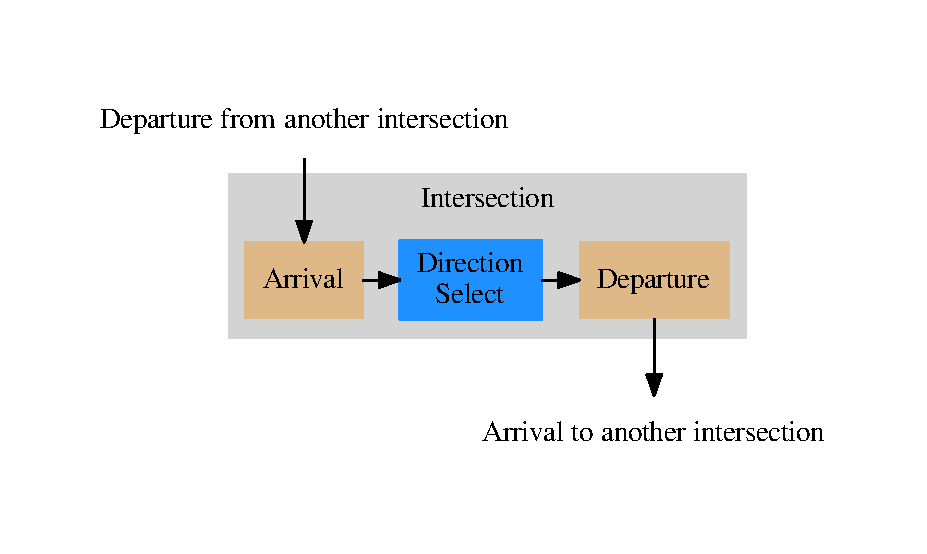
\includegraphics[width=0.6\textwidth]{figs/graphviz/traffic_events.pdf}
    \caption{Intersection Event Sequence}\label{traffic_events}
\end{figure}

All events in the traffic model follow an exponential distribution and a single event
is generated with the processing of each event. The departure and direction select events
are self-generated but the arrival event is from an adjacent intersection.

\subsection{Epidemic}

The epidemic model describes the spreading of an infectious disease across a set of
geographic locations in a region and across a set of regions. The logical processes in
the simulation are geographic locations which represent a portion of the population. The
interactions between people in different geographic locations and regions are modeled with
a diffusion network. An abstract view of the simulation model is shown below in figure
\ref{epidemic_model}.

\begin{figure}[H]
    \centering
    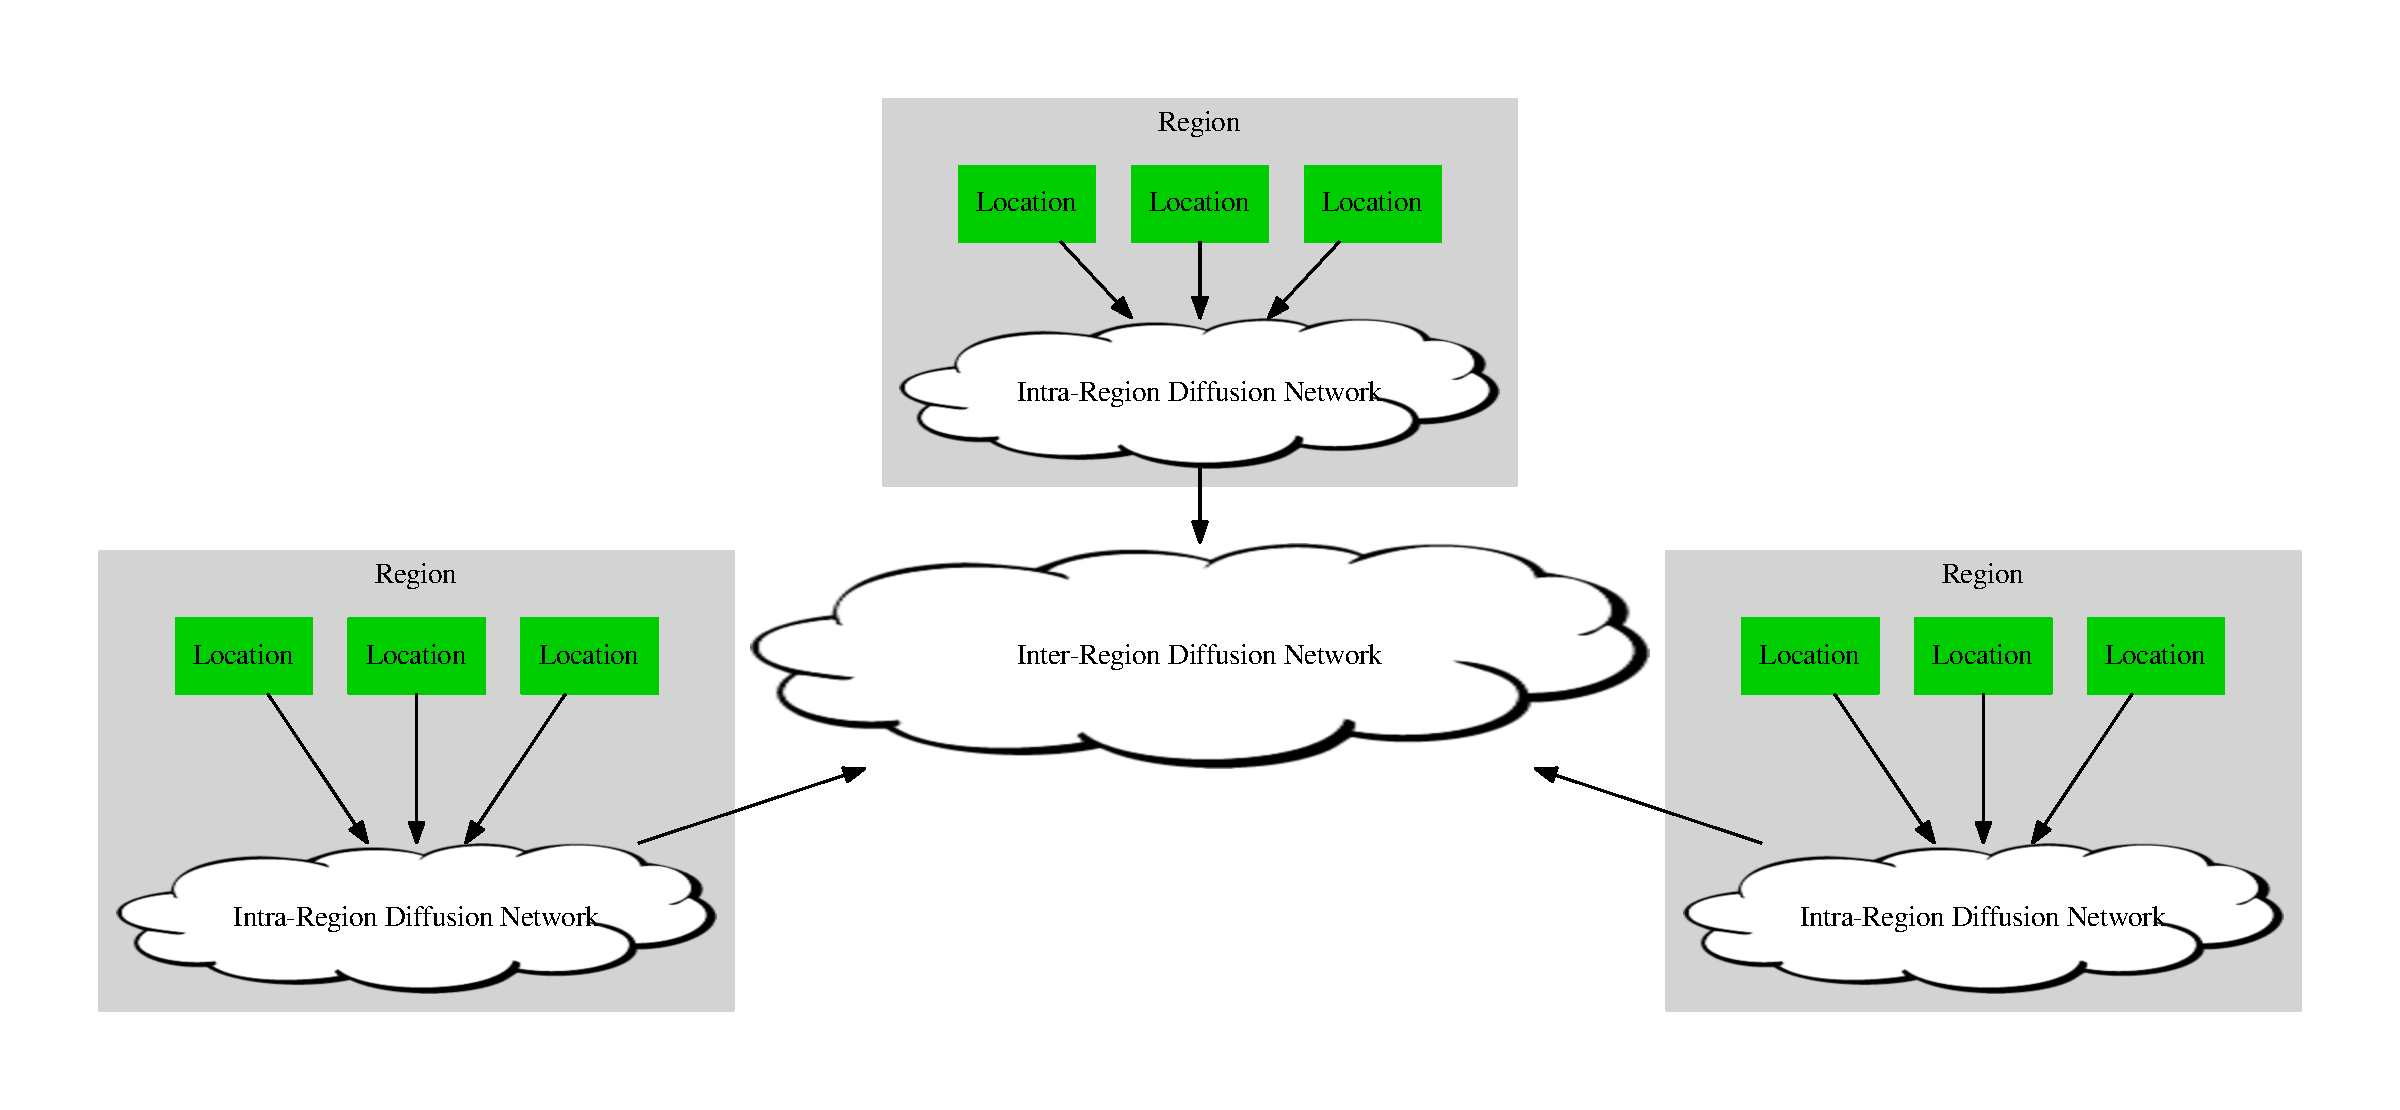
\includegraphics[width=0.6\textwidth]{figs/graphviz/epidemic.pdf}
    \caption{Epidemic Model}\label{epidemic_model}
\end{figure}

The model is based on reaction-diffusion model\cite{perumalla-12}. The reaction process
models the behavior of the disease within a person as well as the transmission of the
disease between people within the same location. A probabilistic reaction function defines
the behavior of the disease between individuals\cite{barrett-08}. The disease within an
individual is modeled by a Probabilistic Timed Transition System (PTTS)\cite{barrett-08}
which is a finite state machine describing the disease states and transitions between states.
Together, the interhost and intrahost models of the disease form the \emph{disease model}.
The diffusion network models the social interactions of people between locations and between
region\cite{barrett-08}.

\subsection{Airport}

The airport model describes the departure and arrivals of airplanes between a connected
set of airports. The logical processes represent airports and the events are simply
departures and arrivals. For simplicity, the airports are connected in a rectangular grid
and can only fly to aiports to the north, east, south, or west of the aiport departed from.
The time spent between takeoff and landing and between landing and takeoff both follow an
exponential distributions.

\section{State Saving}

Figure \ref{ssp_analysis_smp} shows the speedup and percent memory decrease over copy state saving
with increasing state saving periods. The memory usage measurements were obtained from malloc
statistics so they only account for heap memory.  All runs were configured for a GVT calculation
period of 100ms, 10 worker threads and 10 LTSF Queues. 

\begin{figure}
  \begin{minipage}{.5\textwidth}
    \begin{center}
      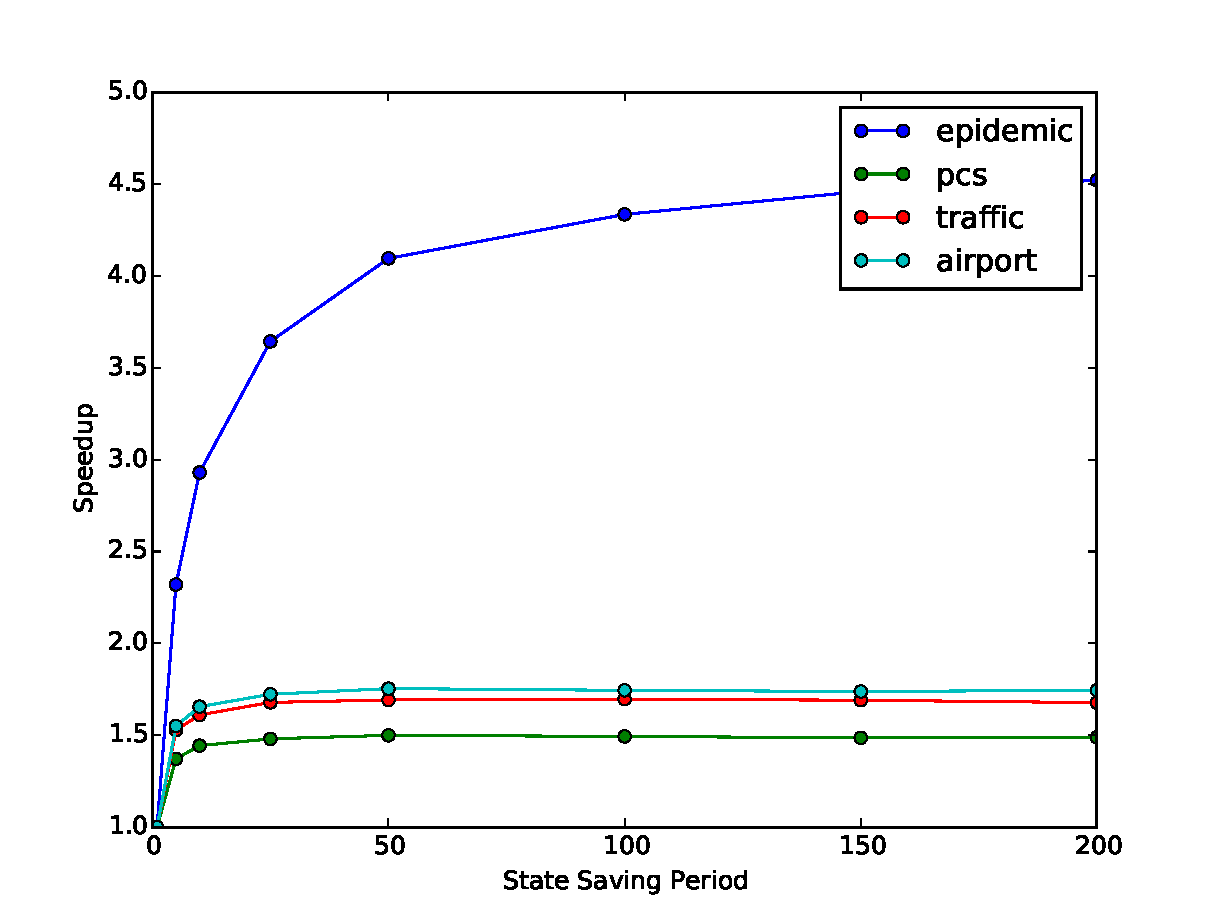
\includegraphics[width=\textwidth,keepaspectratio]{figs/state_saving/speedup.pdf} \\
      Speedup \\
    \end{center}
  \end{minipage} \hfill
  \begin{minipage}{.5\textwidth}
    \begin{center}
      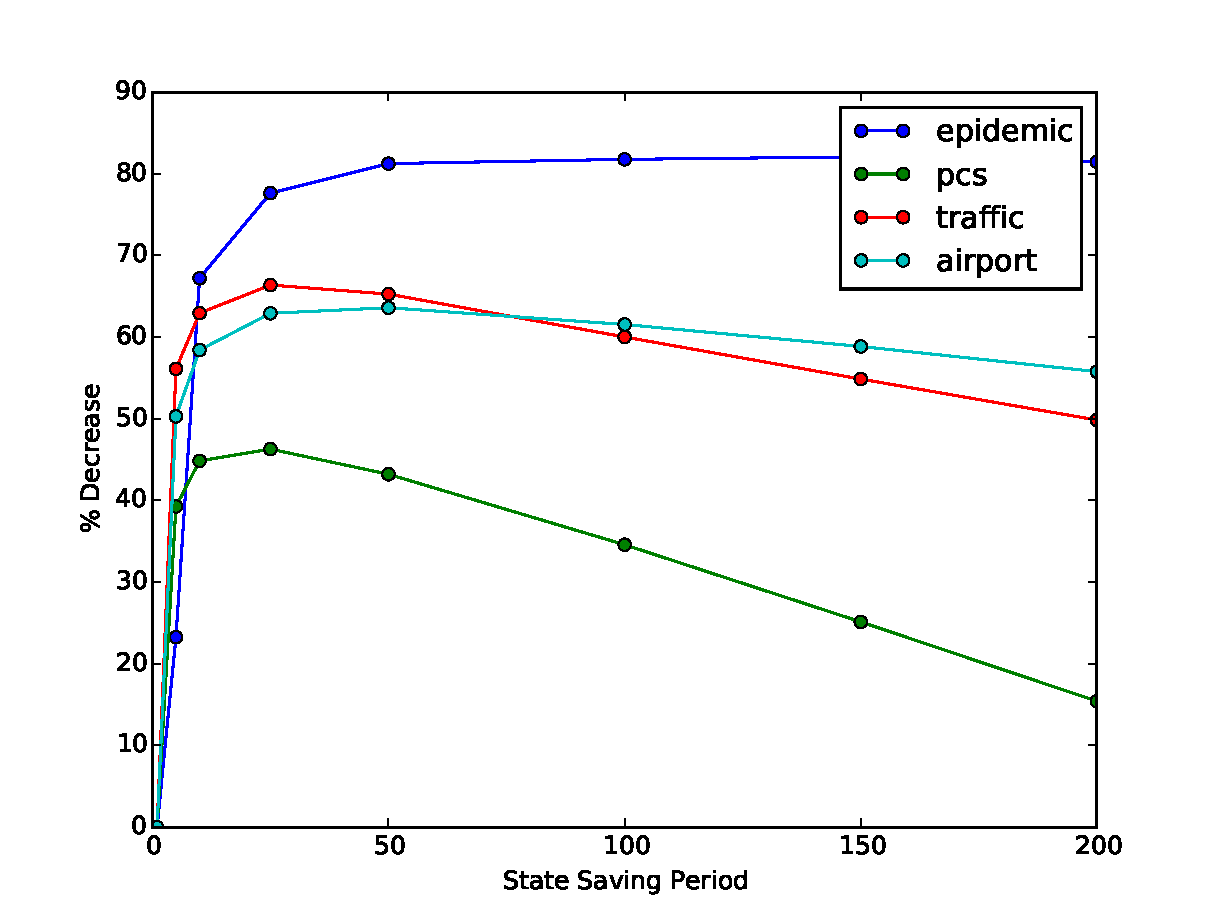
\includegraphics[width=\textwidth,keepaspectratio]{figs/state_saving/percent_memory_decrease.pdf} \\
      Percent Decrease in Peak Memory \\
    \end{center}
  \end{minipage}
  \caption{Periodic State Saving on SMP Machine}\label{ssp_analysis_smp}
\end{figure}

It is apparent that benefits of increasing the state saving period are huge for lower periods
due to less copying and lower memory requirements. However, with larger periods the increased
rollback length will start to counteract. The time to rollback will take longer due to longer
coaster forwarding phases and the memory requirements will increase due to the extra processed
events saved for coast forwarding. The increased rollback time doesn't seem to make much difference
even at large periods but the memory footprint increases linearly so the ideal period should be
the point at which the memory requirements are the lowest. The ideal period will be different
for all models because it will depend on the relative size of the events and states. The period
for the PCS, Traffic, and Airport models appears to be the best around 25 but for the Epidemic
model which has a large state to event ratio will be much larger.

\section{Fossil Collection}

There are two ways that fossil collection can be achieved in \textsc{warped2}. The first way
is to have the worker threads fossil collect one LP at a time as they process events. The last
fossil collect time can be recorded for each LP so that the worker threads can know when fossil
collection is needed by comparing the times to the current GVT. The second way is to have the
manager thread fossil collect all LPs. Once the GVT is calculated, all LPs can be fossil collected
all at once.

With manager thread fossil collection, the worker threads are relieved from unnecessary work
that can slow down event processing but extra locks will be needed to protect access to the
processed queue, output queue, and state queue for each LP. Worker thread fossil collection
will be the more scalable approach for both the number of LPs and the number of processes since
the manager thread must perform other tasks such as GVT and interprocess communication.

Figure \ref{fc_times} 

\begin{figure}
  \begin{minipage}{.5\textwidth}
    \begin{center}
      \begin{tabular}{| c | c |}
        \hline
        Model   & Maximum Time \\
        \hline
        PCS     & 10,000  \\
        Traffic & 100,000 \\
        Epidemic& 100,000 \\
        Airport & 100,000 \\
        \hline
      \end{tabular}
    \end{center}
  \end{minipage} \hfill
  \begin{minipage}{.5\textwidth}
    \begin{center}
      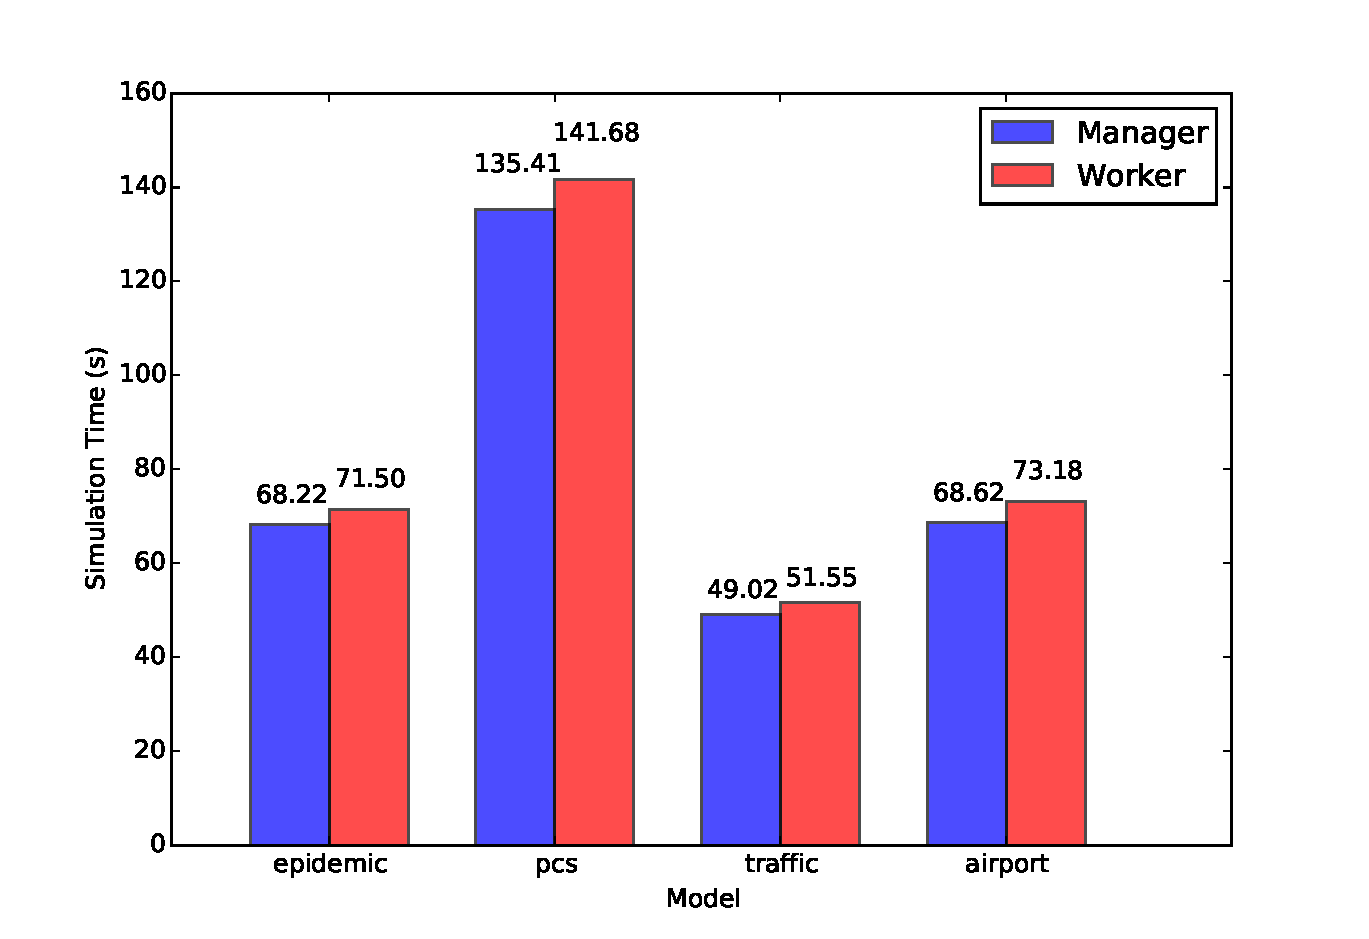
\includegraphics[width=\textwidth]{figs/fossil_collection/simulation_times.pdf}
    \end{center}
  \end{minipage}
  \caption{Performance Comparison for Fossil Collection Methods}\label{fc_times}
\end{figure}


\begin{figure}
  \begin{minipage}{.5\textwidth}
    \begin{center}
      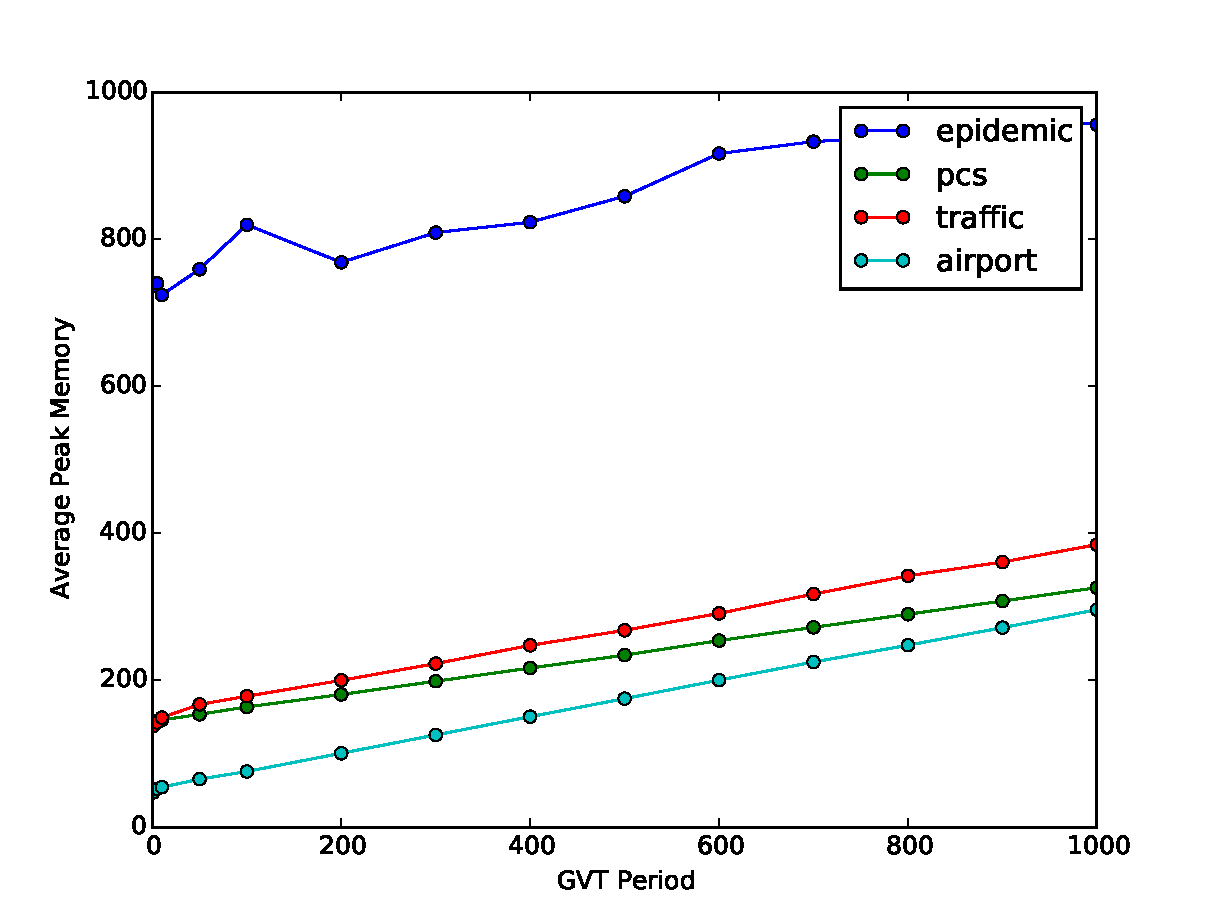
\includegraphics[width=\textwidth,keepaspectratio]{figs/fossil_collection/memory_fcw.pdf} \\
      Worker Threads \\
    \end{center}
  \end{minipage} \hfill
  \begin{minipage}{.5\textwidth}
    \begin{center}
      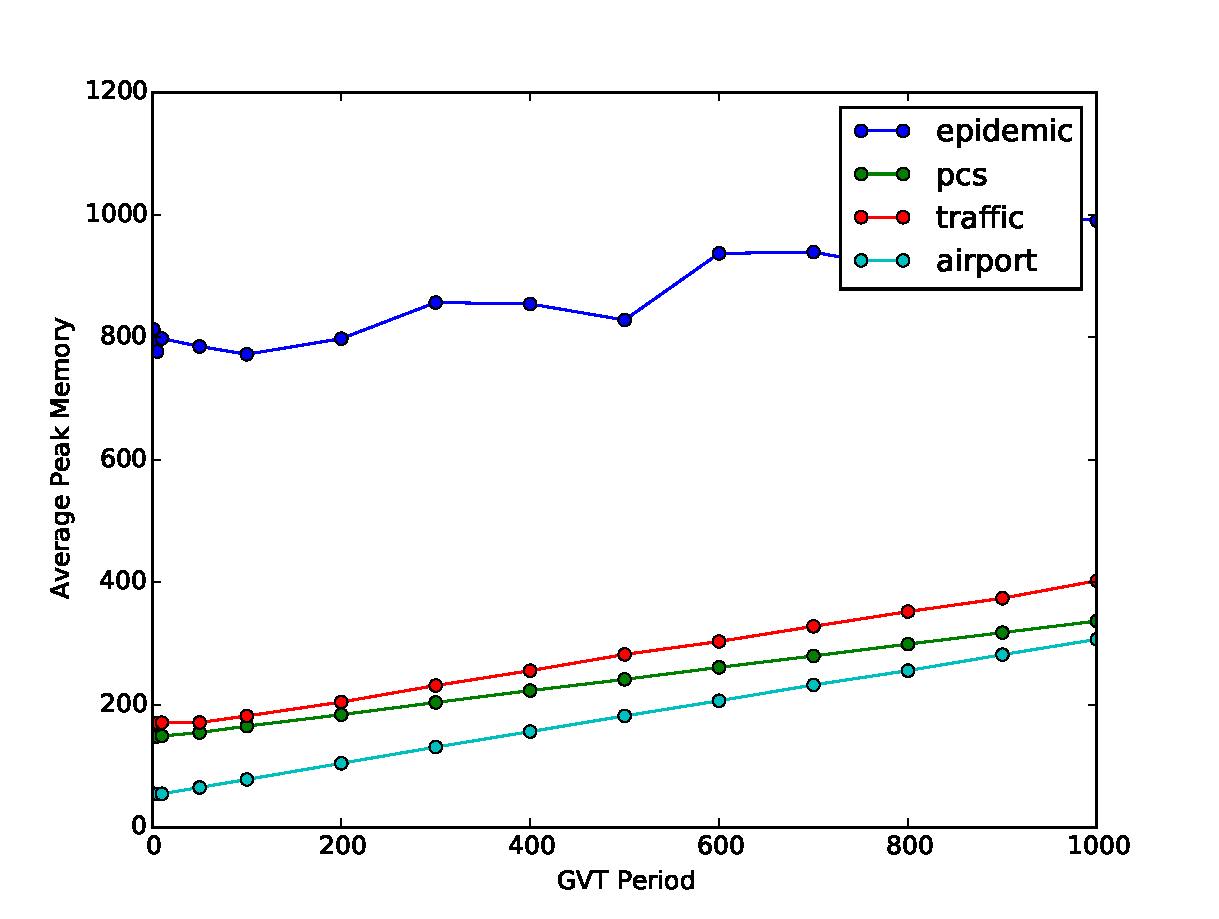
\includegraphics[width=\textwidth,keepaspectratio]{figs/fossil_collection/memory_fcm.pdf} \\
      Manager Thread \\
    \end{center}
  \end{minipage}
  \caption{Memory Comparison for Fossil Collection Methods}\label{fc_memory_analysis}
\end{figure}

\section{Pending Event Set}

\subsection{LTSF Queues}

\begin{figure}
  \begin{minipage}{.5\textwidth}
    \begin{center}
      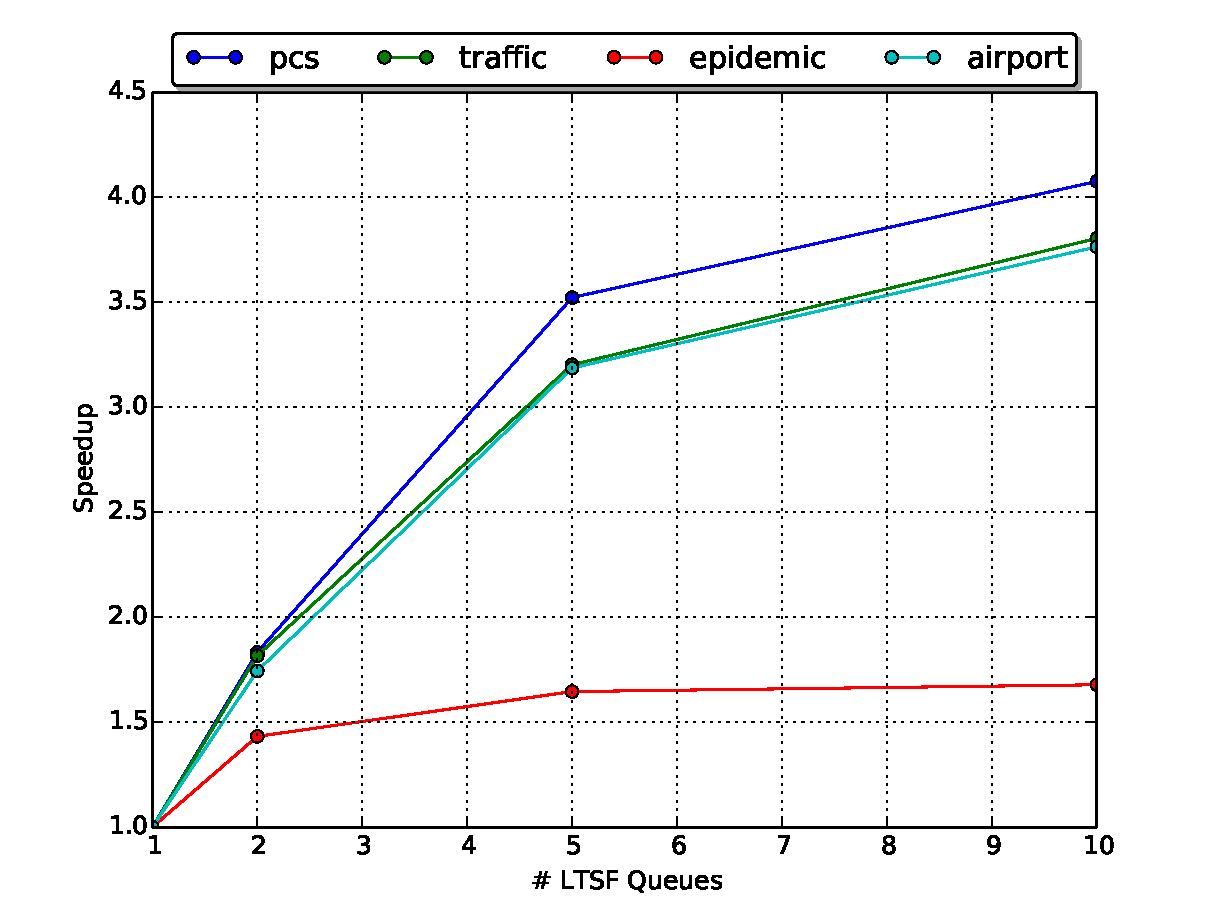
\includegraphics[width=\textwidth,keepaspectratio]{figs/pending_event_set/ltsf_speedup.pdf} \\
      Speedup \\
    \end{center}
  \end{minipage} \hfill
  \begin{minipage}{.5\textwidth}
    \begin{center}
      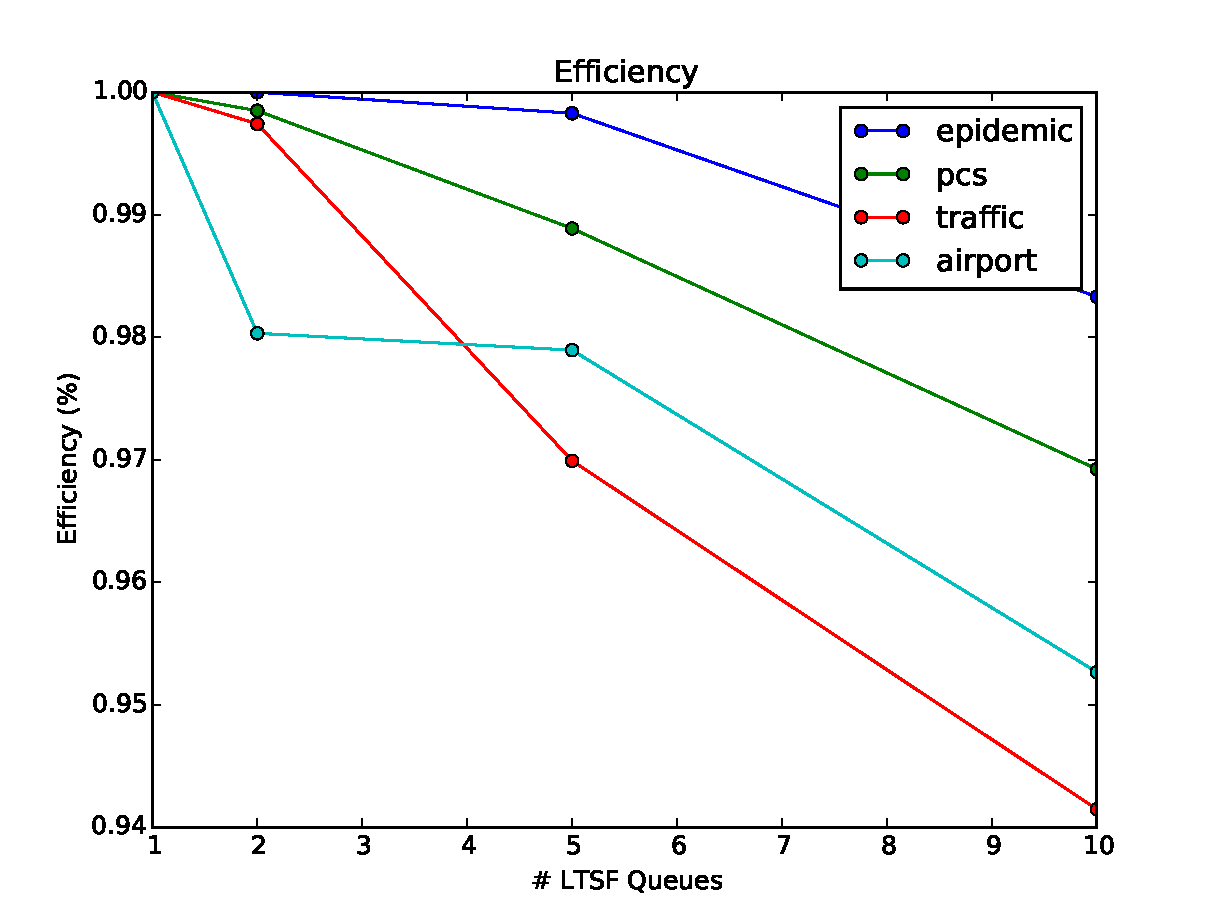
\includegraphics[width=\textwidth,keepaspectratio]{figs/pending_event_set/ltsf_efficiency.pdf} \\
      Efficiency \\
    \end{center}
  \end{minipage}
  \caption{LTSF Queues}\label{ltsf_analysis}
\end{figure}

%% Explain results
From these results it is apparent that contention to the LTSF queues outweigh the extra time
needed to process a larger number of rollbacks.

%%TODO  ^ ^ ^ ^ ^ ^ ^ ^
%%TODO  | | | | | | | |

%%TODO, possibly mention this in future research

\subsection{Spinlocks}

\begin{figure}
\centering
  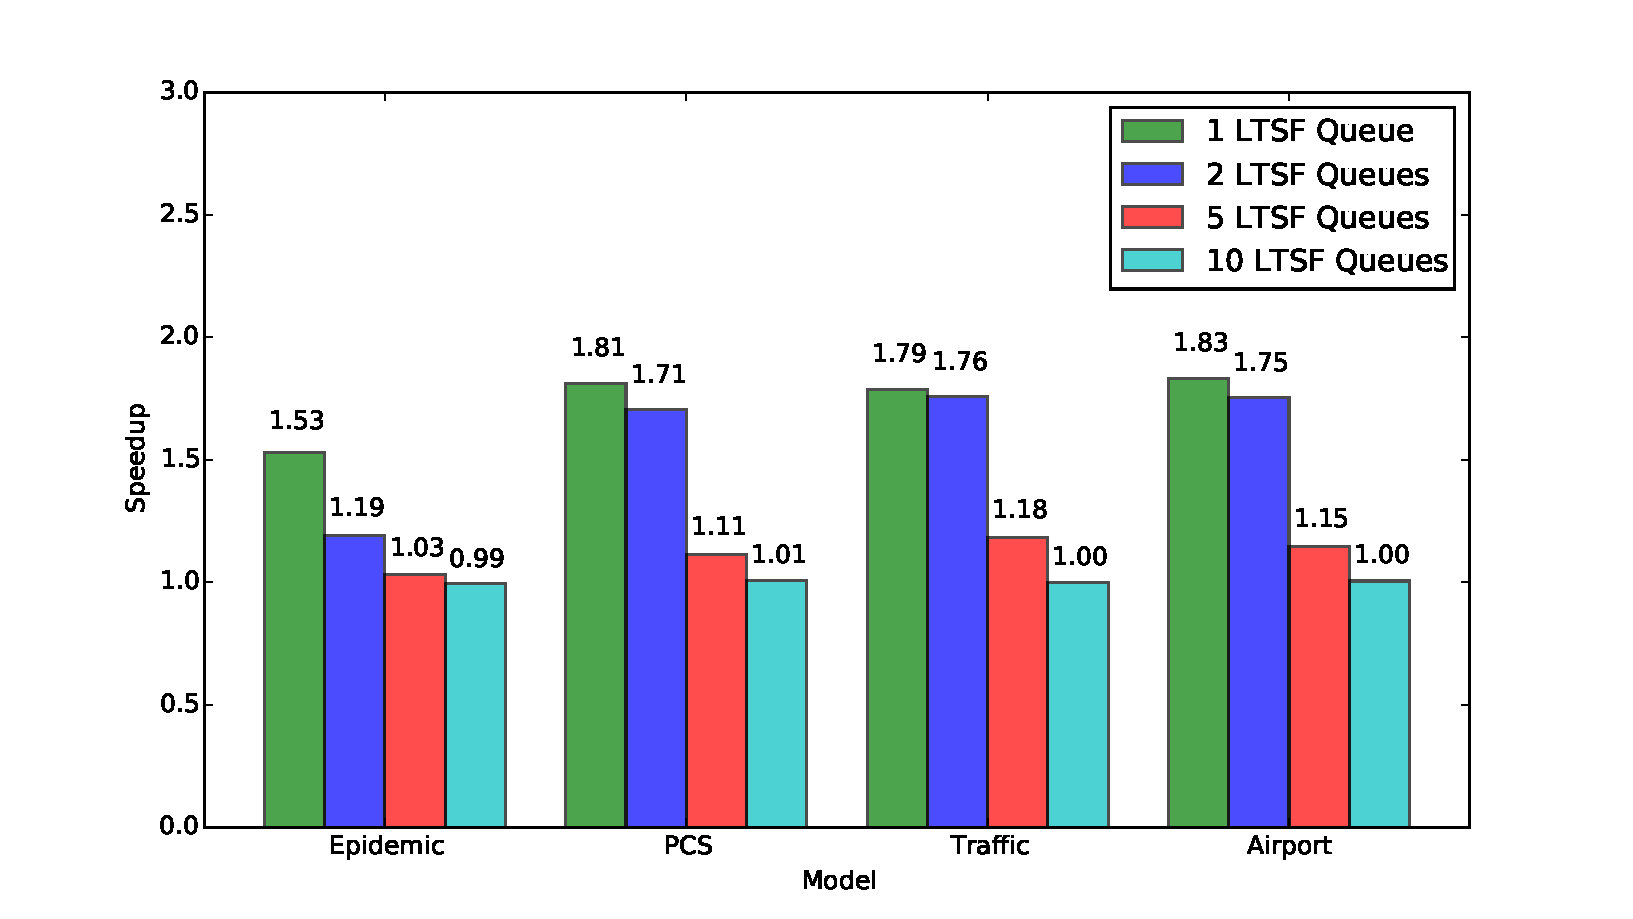
\includegraphics[width=0.5\textwidth]{figs/pending_event_set/spinlock_speedup.pdf}
\end{figure}

\section{Partitioning}


\section{Memory Allocation}

\subsection{Thread-Caching Malloc (TCMalloc)}

TCMalloc is a memory allocator that is designed to efficiently allocate memory in
multi-threaded applications such as \textsc{warped2}. In TCMalloc, seperate thread-local
caches of free memory are maintained to avoid contention that would be caused by shared
caches.

\chapter{ARM big.LITTLE Platform}\label{big_little_platform}

\pagebreak

\begin{table}
    \centering
    \begin{tabular}{|| l | l | c c ||}
    \hline
        \multicolumn{2}{|l|}{} & \multicolumn{2}{c||}{Exynos 5422} \\ \cline{3-4}
        \multicolumn{2}{|l|}{} & Cortex-A15 & Cortex-A7 \\ [0.5ex]
        \hline\hline
        \multirow{8}{*}{Processor}
            & ISA           & \multicolumn{2}{c||}{ARMv7} \\
            & \# Cores      & 4         & 4 \\
            & \# Threads    & \multicolumn{2}{c||}{8} \\
            & Frequency     & 2.0 GHz   & 1.4 GHz \\
            & L1 Data Cache & 32kB      & 32kB \\
            & L1 Inst Cache & 32kB      & 32kB \\
            & L2 Cache      & 2MB       & 512kB\\
        \hline
        \multirow{2}{*}{Memory}
            & Type          & \multicolumn{2}{c||}{2 x LPDDR3-933} \\
            & Max Bandwidth & \multicolumn{2}{c||}{14.9 GB/s} \\
        \hline
        \multirow{2}{*}{Runtime}
            & Compiler      & \multicolumn{2}{c||}{?} \\
            & MPI Version   & \multicolumn{2}{c||}{?} \\
        \hline
    \end{tabular}
    \caption{ODROID XU3 Platforms}\label{odroid_platform}
\end{table}

\section{Load Distribution}

\section{CPU Affinity}

\section{Large Page Size}

\section{Memory Bandwidth Benchmarks}

\chapter[Conclusions \& Future Research]{Conclusions and Suggestions for Future Research}
\label{conclude}

\section{Summary of Findings}

\section{Detailed Conclusions}

\section{Suggestions for Future Work}

%%\Appendix
%%\chapter{Appendix A}\label{appendixA}


\bibliography{refs}
\bibliographystyle{ieeetr} \markright{ }

\end{document}
